\chapter{点扫描显微镜系统设计的理论基础}\label{chap:2}
\section{点扫描显微系统设计中的速度和分辨率问题}\label{2.1}
点扫描显微镜(point-scanning microscopy)是指利用高度聚焦的激发光束在样品上按预定轨迹逐点扫描，并将各扫描位置对应的探测信号按照空间坐标重建为二维或三维图像的一类显微成像方式。与宽场显微成像中``整个视场同时照明、相机并行探测''不同，点扫描显微镜在任一时刻只激发样品中的一个局部体积元，因此其成像速度、信噪比和空间分辨率均与扫描方式、像素停留时间以及激发光参数密切相关。

本章围绕多光子荧光寿命成像系统构建所展开的统一设计基础。由于后续第三章中的共聚焦荧光寿命显微镜、第四章中的多光子显微平台以及第五章中的荧光寿命同步采集与图像重建，均建立在点扫描成像框架之上，因此有必要首先从像素停留时间、采样分辨率、扫描视场、点扩散函数以及有效激发体积等基本问题出发，分析扫描速度、空间分辨率、信噪比与视场范围之间的内在制约关系。通过本章建立的理论框架，后续各章中涉及的扫描结构选择、光路参数配置、脉冲激发条件以及寿命数据采集策略，均能够被放置在统一的系统设计逻辑下理解。

点扫描显微镜通常包括激光扫描共聚焦显微镜、多光子显微镜等形式。其主要特点在于：一方面，通过逐点激发和逐点探测，可以有效抑制离焦背景，提高成像对比度，并结合针孔或非线性激发实现三维光学切片；另一方面，由于图像是通过逐点累积形成的，单个像素能够获得的信号量受像素停留时间限制，因此系统帧率、视场大小与信噪比之间往往需要进行折中设计。

\subsection{点扫描的单像素停留时间}\label{2.1.1}
与宽场成像方式不同，点扫描成像采用逐点或逐像素扫描的方式获取图像。在理想情况下，若一帧图像的总采集时间为 $T_{\mathrm{frame}}$，图像总像素数为 $N$，则单个像素的平均停留时间可表示为

\begin{equation}
T_0=\frac{T_{\mathrm{frame}}}{N}
\label{eq:dwell_time_basic}
\end{equation}

其中，$N=N_xN_y$，$N_x$ 和 $N_y$ 分别表示图像在两个方向上的采样像素数。

相比之下，在宽场成像系统中，所有像素在同一曝光时间内同时积分，因此单个像素的有效曝光时间近似满足

\begin{equation}
T_0^{(\mathrm{widefield})}=T_{\mathrm{frame}}
\label{eq:widefield_exposure}
\end{equation}

以 $512\times512$ 像素图像为例，在保持相同帧率条件下，宽场成像中单个像素的有效曝光时间约为点扫描模式的$512\times512=2.62\times10^{5}$倍。由此可见，点扫描成像中单像素可积累信号的时间远短于宽场成像，因此更容易受到光子统计噪声的限制。

在点扫描成像中，若不区分具体激发机制，仅从经验上讨论单像素信号强度与停留时间的关系，则单个像素获得的总信号可写为

\begin{equation}
I \propto \eta \,\beta \,T_0\, S_{\mathrm{exc}}
\label{eq:signal_general}
\end{equation}

其中，$\eta$ 表示系统的综合探测效率，$\beta$ 表示样品的发光效率，$T_0$ 为单像素停留时间，$S_{\mathrm{exc}}$ 表示激发强度相关项。该式表明，在其他条件不变时，单像素信号与停留时间近似成正比。

对于脉冲激光激发，激发强度不仅与平均功率有关，还与单脉冲能量、脉冲宽度和重复频率等有关。特别是在多光子激发条件下，荧光信号对峰值功率具有非线性依赖关系，因此缩短脉冲宽度、提高单脉冲能量通常有利于提高激发效率。

此外，若考虑扫描回扫、加减速和同步控制等实际开销，式~(\ref{eq:dwell_time_basic}) 仅为理想情况下的近似表达。实际系统中的有效像素停留时间通常还与扫描占空比、行周期和控制方式有关。

假设单个像素存在最小有效停留时间 $T_{0,\min}$，则至少应保证在一个像素停留时间内能够接收到不少于一个激发脉冲，即:

\begin{equation}
T_{0,\min}\gtrsim \frac{1}{f}
\label{eq:min_dwell_time}
\end{equation}

其中 $f$ 为激光重复频率。实际上，为了获得稳定的荧光统计信号，通常需要一个像素内包含多个激发脉冲。因此，在提高成像速度的同时，常需要综合优化激光重复频率、扫描速度与像素数等参数。

此外，在帧率保持不变的条件下，如果增大成像幅面尺寸(即视场范围)，同样会导致单个像素的停留时间减少。以Supercontuum 40MHz白光超连续皮秒激光器为例，在Scanimage软件中不同视场尺寸与帧率组合条件下，对应的单像素停留时间以及每个像素所包含的脉冲数量如表\ref{Table2.1}所示。

\begin{table}[htbp]
\bicaption{40MHz激发频率下不同扫描速度和数字化像素数对应的单像素时间以及单像素包含脉冲数关系}{Relationship between pixel dwell time and the number of excitation pulses per pixel at 40~MHz for different scan speeds and digitized pixel numbers}
\label{Table2.1}
\centering
\resizebox{\textwidth}{!}{%
\begin{tabular}{c|c|c|c|c}
\hline
{40MHz重复频率} &
  {128 x 128} &
  {256 x 256} &
  {512 x 512} &
  {1024 x 1024} \\ \hline
{} &
  {单像素时间: 61.04 μs} &
  {单像素时间: 15.26 μs} &
  {单像素时间: 3.81 μs} &
  {单像素时间:   0.954 μs} \\
\multirow{-2}{*}{{1 Hz}} &
  {单像素脉冲数: 2441.4 个} &
  {单像素脉冲数: 610.4 个} &
  {单像素脉冲数: 152.6 个} &
  {单像素脉冲数: 38.1 个} \\ \hline
{} &
  {单像素时间: 6.10 μs} &
  {单像素时间: 1.53 μs} &
  {单像素时间: 381 ns} &
  {单像素时间: 95.4 ns} \\
\multirow{-2}{*}{{10 Hz}} &
  {单像素脉冲数: 244.1 个} &
  {单像素脉冲数: 61.0 个} &
  {单像素脉冲数: 15.3 个} &
  {单像素脉冲数: 3.8 个} \\ \hline
{} &
  {单像素时间: 2.54 μs} &
  {单像素时间: 636 ns} &
  {单像素时间: 159 ns} &
  {单像素时间: 39.7 ns} \\
\multirow{-2}{*}{{24 Hz}} &
  {单像素脉冲数: 101.7 个} &
  {单像素脉冲数: 25.4 个} &
  {单像素脉冲数: 6.4 个} &
  {单像素脉冲数: 1.6 个} \\ \hline
{} &
  {单像素时间: 610 ns} &
  {单像素时间: 153 ns} &
  {单像素时间: 38.1 ns} &
  {单像素时间: 9.5 ns} \\
\multirow{-2}{*}{{100 Hz}} &
  {单像素脉冲数: 24.4 个} &
  {单像素脉冲数: 6.1 个} &
  {单像素脉冲数: 1.5 个} &
  {单像素脉冲数: 0.4 个} \\ \hline
{} &
  {单像素时间: 407 ns} &
  {单像素时间: 102 ns} &
  {单像素时间: 25.4 ns} &
  {单像素时间: 6.4 ns} \\
\multirow{-2}{*}{{150 Hz}} &
  {单像素脉冲数: 16.3 个} &
  {单像素脉冲数: 4.1 个} &
  {单像素脉冲数: 1.0 个} &
  {单像素脉冲数: 0.3 个} \\ \hline
{} &
  {单像素时间: 204 ns} &
  {单像素时间: 50.9 ns} &
  {单像素时间: 12.7 ns} &
  {单像素时间: 3.2 ns} \\
\multirow{-2}{*}{{300 Hz}} &
  \multicolumn{1}{l|}{{单像素脉冲数: 8.2 个}} &
  \multicolumn{1}{l|}{{单像素脉冲数: 2.0 个}} &
  \multicolumn{1}{l|}{{单像素脉冲数: 0.5 个}} &
  \multicolumn{1}{l}{{单像素脉冲数: 0.1 个}} \\ \hline
\end{tabular}%
}
\end{table}



\subsection{点扫描成像的数字采样分辨率}\label{2.1.2}
在点扫描显微成像系统的数字化采样过程中，需要满足香农-奈奎斯特采样定理。即便显微镜本身具有较高的光学分辨率，在数字成像阶段，像素尺寸仍需满足$D_{pixel}<1/2D_{sample}$才能有效分辨目标结构。换言之，数字像素尺寸必须小于待观测结构尺寸的一半。

因此，在相同视场范围(field of view，FOV)条件下，虽然通过减少像素数量可以提高扫描速度，但同时也会降低图像的采样分辨率，从而影响最终成像质量。

\begin{figure}[htbp]
    \centering

    \begin{subfigure}[b]{0.42\textwidth}
        \centering
        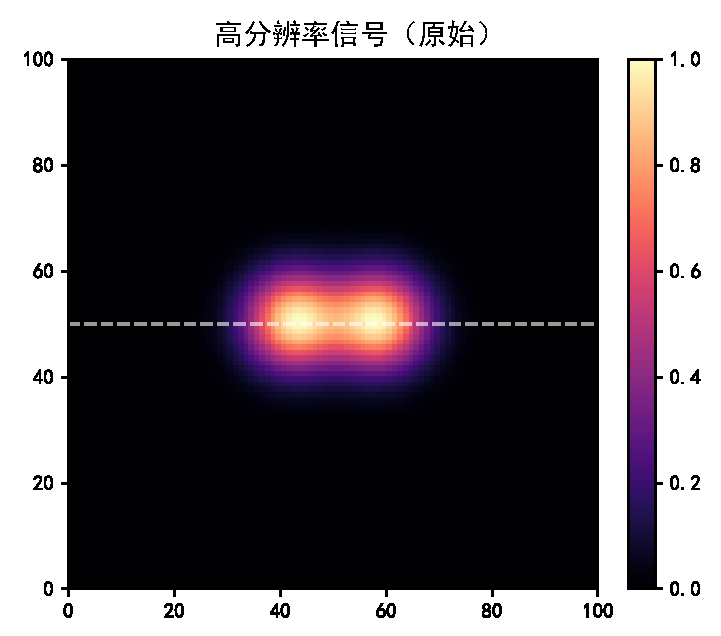
\includegraphics[width=\textwidth]{Fig/Fig03-a.pdf}
        \caption{}
        \label{fig03a}
    \end{subfigure}
    \hfill
    \begin{subfigure}[b]{0.5\textwidth}
        \centering
        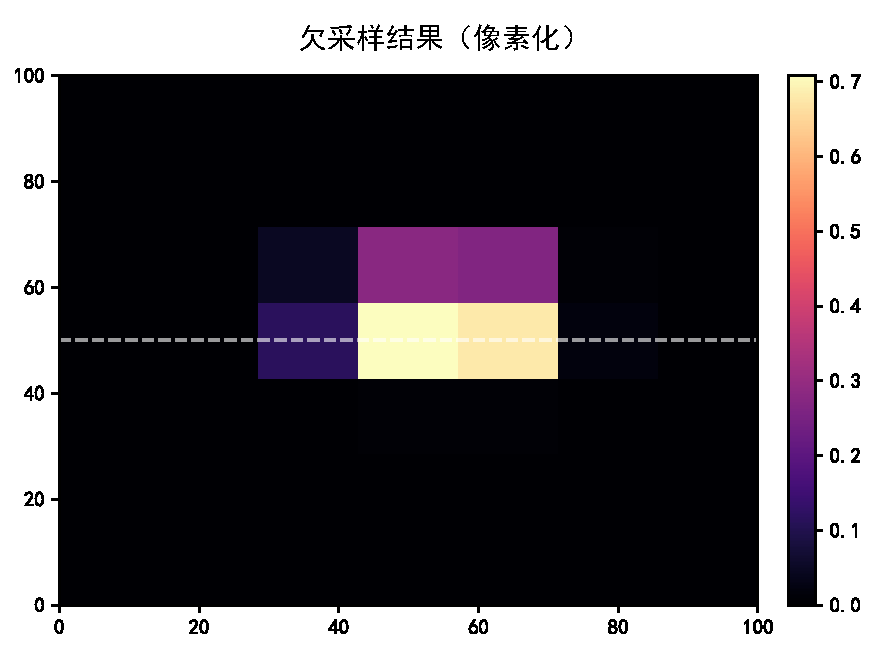
\includegraphics[width=\textwidth]{Fig/Fig03-b.pdf}
        \caption{}
        \label{fig03b}
    \end{subfigure}

    \vspace{0.3cm}

    \begin{subfigure}[b]{0.92\textwidth}
        \centering
        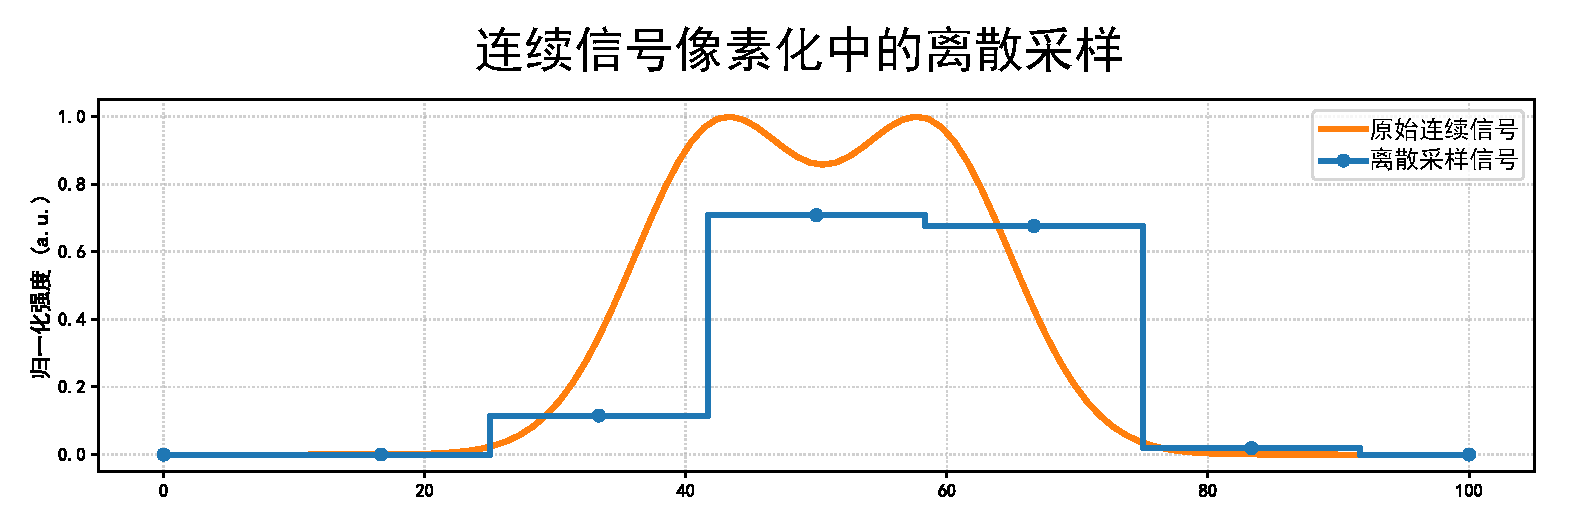
\includegraphics[width=\textwidth]{Fig/Fig03-c.pdf}
        \caption{}
        \label{fig03c}
    \end{subfigure}

    \bicaption{数字化采样对空间分辨率的影响。(a) 高分辨率连续信号的原始分布；(b) 欠采样条件下的像素化结果；(c) 连续信号像素化中的离散采样示意图}
    {Impact of digital sampling on spatial resolution. (a) Original distribution of a high-resolution continuous signal; (b) pixelated result under undersampling; (c) schematic illustration of discrete sampling during pixelization of a continuous signal}
    \label{fig03}
\end{figure}

如图~\ref{fig03}(\subref{fig03a})所示，原始高分辨率连续信号呈现出更丰富的空间细节；图~\ref{fig03}(\subref{fig03b})展示了较大采样间隔下的像素化欠采样结果；图~\ref{fig03}(\subref{fig03c})进一步示意了连续信号的离散采样过程。



\section{点扩散函数}\label{2.2}
点扩散函数(Point Spread Function, PSF)是描述显微成像系统空间响应能力的核心概念。理想情况下，若样品中存在一个空间尺寸远小于系统分辨极限的发光点源，则该点源经过物镜、管镜以及探测系统后，不会在像面上成一个几何点，而会形成具有有限空间展宽的光强分布。该分布即称为点扩散函数。换言之，PSF 描述了``系统如何成像一个点''，而图像(二维结构)正是由一系列点(一维结构)所构成的，因此它直接反映了系统对空间细节的保真能力。

从成像角度看，任意物体都可以视作大量点源的叠加，显微系统获得的图像可理解为物体分布与 PSF 的卷积结果。因此，PSF 越窄，系统越能够区分彼此接近的两个发光点，成像分辨率也越高；反之，PSF 越宽，相邻结构越容易相互重叠，导致细节模糊，所以PSF 的横向与轴向展宽是评价显微系统空间分辨率的重要依据。

对于点扫描显微镜而言，PSF 不仅决定图像分辨率，也决定了每个扫描位置对应的有效激发体积。在共聚焦显微镜中，PSF 的收缩有助于提高光学切片能力；而在多光子显微镜中，由于荧光激发对光强具有非线性依赖，实际参与信号产生的空间区域会比线性激发情形进一步缩小，从而带来更强的空间局域化能力和更低的离焦背景。




\subsection{线性点扩散函数与多光子有效激发体积}\label{2.2.1}
在激发光束充分填充(Overfilling)物镜后孔径且系统像差较小的近似条件下，焦点附近的光强分布可表示为时间项与空间项的乘积形式，即
\begin{equation}
  I(\mathbf{r},t)=I_{0}(t)\,h(\mathbf{r})
  \label{eq:psf_separation}
\end{equation}

其中 $\mathbf{r}=(x,y,z)$ 为空间坐标，$I_{0}(t)$ 表示与入射功率相关的时间项，$h(\mathbf{r})$ 表示归一化的空间强度分布，并满足

\begin{equation}
  0\le h(\mathbf{r})\le 1,\qquad h(\mathbf{0})=1
\end{equation}

这里的 $h(\mathbf{r})$ 即线性激发条件下的强度型点扩散函数。

对于衍射受限聚焦系统，焦点处峰值强度与入射功率、波长及物镜数值孔径有关。在近似讨论中，常可写为

\begin{equation}
  I_{0}(t)\propto \frac{(NA)^2}{\lambda^2}P(t)
  \label{eq:I0_scaling}
\end{equation}

其中 $NA$ 为物镜数值孔径(Numerical Aperture)，$\lambda$ 为激发波长，$P(t)$ 为入射光功率。需要说明的是，式~(\ref{eq:I0_scaling}) 仅表示峰值光强的标度关系，其具体系数与光束类型、后孔径填充程度以及像差情况有关，因此更适合写成比例关系，而不宜在缺少完整推导时直接写成严格等式。

在线性荧光激发条件下，单位体积内的荧光产生率与局域光强近似成正比，因此实际参与成像的空间权重可写为

\begin{equation}
  S_{1}(\mathbf{r})\propto h(\mathbf{r})
  \label{eq:linear_psf}
\end{equation}

对于 $m$ 光子激发过程，局域激发概率与光强的 $m$ 次方成正比，因此多光子显微镜中的有效激发分布应写为

\begin{equation}
  S_{m}(\mathbf{r})\propto [I(\mathbf{r},t)]^{m}
  \propto [I_{0}(t)]^{m}[h(\mathbf{r})]^{m}
  \label{eq:multiphoton_psf}
\end{equation}

若仅关注空间分布，则其归一化形式可写为

\begin{equation}
  \widetilde{S}_{m}(\mathbf{r})\propto [h(\mathbf{r})]^{m}
  \label{eq:effective_psf}
\end{equation}

因此，在双光子和三光子情形下分别有

\begin{equation}
\widetilde{S}_{2}(\mathbf{r})\propto [h(\mathbf{r})]^2\qquad
\widetilde{S}_{3}(\mathbf{r})\propto [h(\mathbf{r})]^3
\end{equation}

上述关系表明，随着非线性阶数升高，有效激发体积将进一步收缩。也就是说，多光子激发并不是简单沿用线性光学中的 PSF，而是由非线性效应将原有空间分布进一步``压窄''。这也是多光子显微镜能够在无需物理针孔的情况下实现较强光学切片能力和背景抑制能力的重要原因。

若进一步将焦点附近的横向强度分布近似为高斯形式：
\begin{equation}
  h(r)\approx \exp\!\left(-\frac{2r^2}{w^2}\right)
  \label{eq:gaussian_psf}
  \end{equation}
  则 $m$ 光子有效激发分布满足
  \begin{equation}
  [h(r)]^m=\exp\!\left(-\frac{2mr^2}{w^2}\right)
  \end{equation}

因此其特征半径缩小为
  \begin{equation}
  w_m=\frac{w}{\sqrt{m}}
  \label{eq:wm_scaling}
\end{equation}

这说明双光子和三光子激发下的有效激发区域相较于单光子情形分别进一步收缩，从而有利于提升空间局域化程度。PSF 的严格表达通常来源于矢量衍射理论，其横向和轴向分布并不完全服从简单高斯函数，实际分析中，常将高斯近似用于定性说明宽度变化规律，而将更精确的横向与轴向分辨率计算建立在衍射理论或数值模拟基础上。

\begin{figure}[htbp]
    \centering
    \begin{subfigure}[b]{0.44\textwidth}
        \centering
        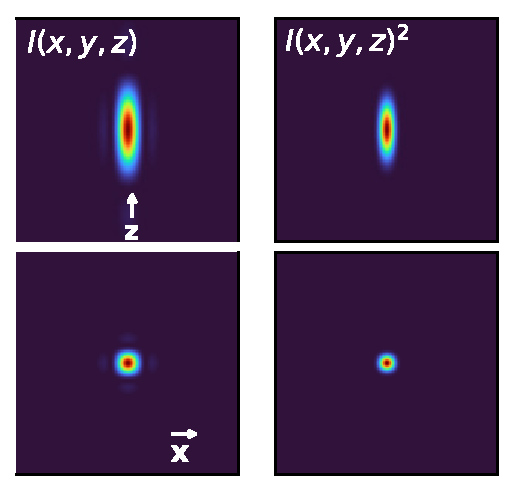
\includegraphics[width=\textwidth]{Fig/Fig07-a.pdf}
        \caption{}
        \label{fig07a}
    \end{subfigure}
    \hfill
    \begin{subfigure}[b]{0.48\textwidth}
        \centering
        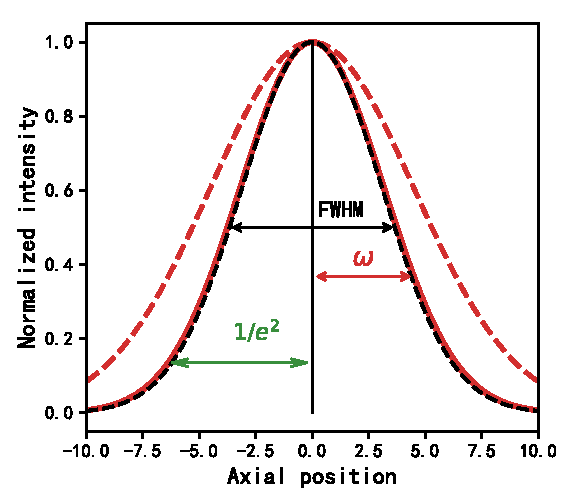
\includegraphics[width=\textwidth]{Fig/Fig07-b.pdf}
        \caption{}
        \label{fig07b}
    \end{subfigure}
    \bicaption{点扩散函数在不同激发条件下的能量分布及其宽度表征参数示意图。(a)线性激发与双光子激发条件下焦点附近能量分布的对比；(b)点扩散函数宽度表征参数示意图}
    {Schematic of the energy distribution of the point spread function under different excitation conditions and its width metrics. (a) Comparison of the energy distribution near focus under linear and two-photon excitation; (b) schematic of the width metrics used to characterize the point spread function}
    \label{fig07}
\end{figure}


如图~\ref{fig07}(\subref{fig07a})\cite{RN1177} 所示，在线性激发与双光子激发条件下，焦点附近的能量分布存在明显差异。左侧两幅图分别表示线性强度分布 $I(x,y,z)$ 在轴向和横向截面上的形态，右侧两幅图表示对应的平方分布 $I^2(x,y,z)$。可以看出，经过非线性激发后，主瓣范围明显缩小，尤其在轴向方向上的压缩更加显著，这意味着只有更靠近焦点中心的区域能够有效产生荧光信号。

图~\ref{fig07}(\subref{fig07b}) 则示意了描述点扩散函数宽度的几种常用指标。其中，FWHM 表示强度下降到峰值一半时对应的全宽，$\omega$ 通常表示高斯分布中 $1/e^2$ 强度位置对应的特征半径。对于高斯函数而言，这些宽度定义虽然在数值上不同，但都可用于表征聚焦光斑或点扩散函数的空间尺度。

在多光子成像中，荧光信号不仅与空间 PSF 有关，还与脉冲激光的时间结构密切相关。对于重复频率为 $f_{\mathrm{rep}}$、脉冲宽度为 $\tau$ 的超短脉冲激光，在平均功率固定时，峰值功率大致与

\begin{equation}
  P_{\mathrm{peak}}\propto \frac{P_{\mathrm{avg}}}{f_{\mathrm{rep}}\tau}
  \label{eq:peak_power_scaling}
\end{equation}
成正比。因此，多光子荧光信号在标度上可近似写为

\begin{equation}
  F_m \propto \eta\,\phi\,C\,\delta_m
  \frac{P_{\mathrm{avg}}^{\,m}}{f_{\mathrm{rep}}^{\,m-1}\tau^{\,m-1}}
  \int [h(\mathbf{r})]^m\,\mathrm{d}V
  \label{eq:m_signal_scaling}
\end{equation}

其中 $\phi$ 为荧光量子产率，$\eta$ 为系统探测效率，$C$ 为荧光分子浓度，$\delta_m$ 为 $m$ 光子吸收截面，$f_{\mathrm{rep}}$ 为激光重复频率，$\tau$ 为脉冲宽度。式~(\ref{eq:m_signal_scaling}) 表明，多光子信号随平均功率呈 $m$ 次幂增长，同时受脉冲宽度、重复频率以及有效激发体积共同影响。

因此，在染料种类与浓度固定、探测链路基本不变的条件下，双光子信号近似与平均功率平方成正比，而三光子信号近似与平均功率立方成正比。而式~\ref{eq:peak_power_scaling}分子中的平均功率受限于组织或样本的热损伤、荧光的热漂白等影响无法无限增加，因此分母$f\tau$对多光子效应成像效果贡献为优化的高优先级，具体推导请查看第~\ref{4.1}节。与此同时，更高的有效数值孔径通常会带来更强的聚焦能力和更小的有效激发体积，从而提高局域激发效率。但这种依赖关系通常通过式~(\ref{eq:I0_scaling}) 和式~(\ref{eq:m_signal_scaling}) 间接体现，而不宜在缺少统一推导前直接写成简单的 $NA^2$ 或更高次幂形式。

综上所述，点扩散函数刻画了显微系统对点源的空间响应，是连接系统分辨率、光学切片能力和多光子有效激发体积的关键物理量。在线性激发条件下，PSF 直接决定成像模糊尺度；而在多光子激发条件下，非线性效应使有效激发分布进一步收缩，从而在提升空间局域化和抑制离焦背景方面展现出显著优势。



\subsection{PSF 宽度指标与分辨率表述}\label{2.2.2}
为了定量描述显微系统的空间分辨能力，通常需要对点扩散函数在横向与轴向上的展宽程度进行表征。常用指标包括半高全宽(full width at half maximum, FWHM)以及高斯近似下的特征半径。本文采用高斯光强分布的常见写法

\begin{equation}
  I(r)=I_0\exp\!\left(-\frac{2r^2}{\omega^2}\right)
  \label{eq:gaussian_width_def}
\end{equation}

其中 $\omega$ 表示光强下降到峰值 $1/e^2$ 时对应的特征半径。对于该定义，FWHM 与 $\omega$ 的关系为

\begin{equation}
  \mathrm{FWHM}=\sqrt{2\ln 2}\,\omega
  \label{eq:fwhm_omega_relation}
\end{equation}

需要指出的是，不同文献中也常采用 $1/e$ 半径或标准差等参数表征高斯宽度，因此在比较不同结果时，必须首先确认所采用的宽度定义是否一致。

在多光子显微镜中，由于有效激发分布满足
\begin{equation}
  \widetilde S_m(\mathbf r)\propto [h(\mathbf r)]^m
\end{equation}

若进一步采用高斯近似，则 $m$ 光子激发下的特征宽度相较于线性激发将缩小为原来的 $1/\sqrt m$。因此，对于双光子激发，有

\begin{equation}
  \omega_{xy}^{(2)}=\frac{\omega_{xy}^{(1)}}{\sqrt2} \qquad
  \omega_{z}^{(2)}=\frac{\omega_{z}^{(1)}}{\sqrt2}
  \label{eq:2p_width_scaling}
\end{equation}

其中 $\omega_{xy}^{(1)}$ 和 $\omega_{z}^{(1)}$ 分别表示线性激发条件下的横向与轴向特征宽度，$\omega_{xy}^{(2)}$ 和 $\omega_{z}^{(2)}$ 则表示双光子激发对应的有效激发宽度。

若采用衍射受限聚焦系统的近似标度关系，并以 $NA_{\mathrm{eff}}$ 表征样品处的有效聚焦能力，则线性激发条件下的横向与轴向宽度通常分别满足

\begin{equation}
  \omega_{xy}^{(1)} \propto \frac{\lambda}{NA_{\mathrm{eff}}}
  \qquad
  \omega_{z}^{(1)} \propto \frac{\lambda}{\,n_0-\sqrt{n_0^2-NA_{\mathrm{eff}}^2}\,}
  \label{eq:linear_width_scaling}
\end{equation}

其中 $\lambda$ 为激发波长，$n_0$ 为样品介质折射率。由式~(\ref{eq:2p_width_scaling}) 可知，双光子激发下对应宽度在此基础上进一步缩小约 $\sqrt2$ 倍。

$NA_{\mathrm{eff}}$ 用于表征后孔径填充不足、系统像差以及折射率失配等因素导致的有效聚焦能力下降。相较于横向宽度，轴向宽度通常对 $NA_{\mathrm{eff}}$ 和折射率失配更为敏感，因此在深层组织成像或介质界面较复杂的场景中，轴向分辨率往往更容易劣化。PSF 的横向与轴向宽度为显微系统分辨率提供了直接表征；而在多光子激发条件下，由于非线性效应引起的有效激发分布收缩，使得系统在空间局域化和离焦背景抑制方面进一步优于线性激发情形。



\section{点扫描成像中的扫描结构}\label{2.3}
激光输出后需经由光束整形与传输光路以保证光束质量、指向稳定性及后续扫描的像差控制。常见的扫描中继结构由扫描透镜(Scan lens, SL)与管透镜(Tube lens, TL)构成：SL 用于在扫描角变化时尽量保持像面平坦并减小光斑畸变，TL 作为成像透镜形成无限远校正系统。对于点扫描多光子显微而言，SL 与 TL 通常构成扫描器到物镜后瞳的光束中继(常等效为4f结构)，其关键目标是将扫描枢轴(pivot)共轭到物镜入瞳，使扫描主要表现为入瞳角度变化而非入瞳位置漂移(非远心扫描)，从而在整个视场内维持接近一致的照明条件与成像质量；同时通过扩束使光束充分填充物镜后孔径，以接近衍射受限聚焦性能。



\subsection{扫描策略：光束扫描与载物台扫描}\label{2.3.1}
显微扫描实现路径通常分为两类：光束扫描与载物台扫描。光束扫描保持样品位置不变，通过改变入射光束角度实现焦点在样品平面内的快速位移，典型执行器包括振镜、共振扫描镜、MEMS 扫描镜、声光偏转器等；载物台扫描保持光束位置固定，通过三维位移平台驱动样品运动实现成像。

两者相比，载物台扫描在大范围拼接或高稳定长时程实验中更具优势，但受限于机械惯量，其瞬态速度通常不及光束扫描。并且在生物活体成像中通常需要生物组织保持相对静止，因此多光子显微系统普遍采用光束扫描作为二维(或三维)成像的基础方案。

\begin{figure}[htbp]
    \centering
    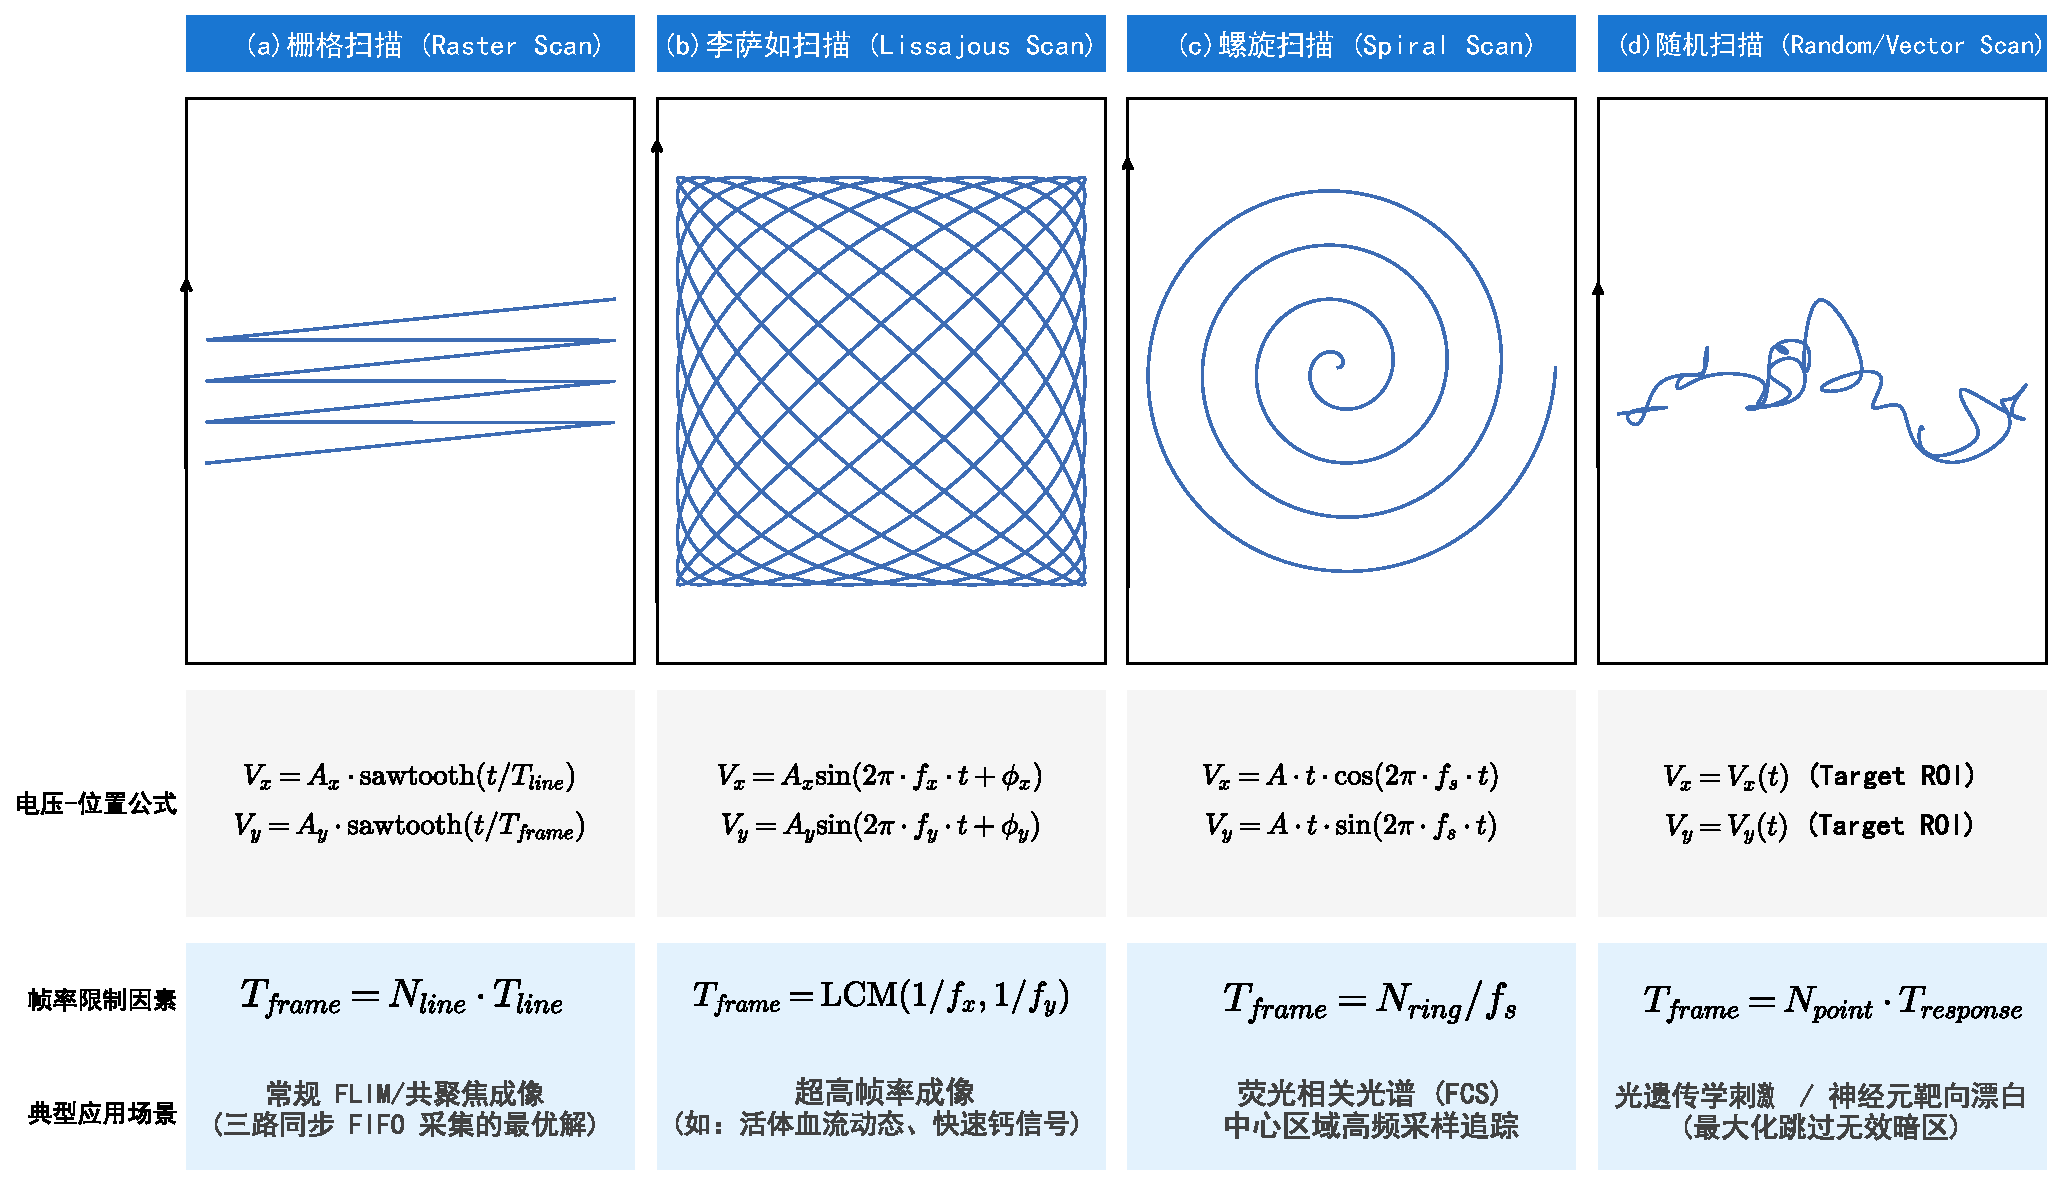
\includegraphics[width=0.8\textwidth]{Fig/Fig08.pdf}
    \bicaption{点扫描中四种代表性扫描轨迹}{Four representative scanning trajectories in point-scanning microscopy}
    \label{fig08}
\end{figure}

如图~\ref{fig08}所示，点扫描显微成像中常见的扫描轨迹主要包括四类。图~\ref{fig08}(a)为栅格扫描(Raster Scan)，通过快慢轴锯齿波驱动实现规则、均匀的全画幅覆盖，是常规共聚焦和荧光寿命成像(FLIM)中最常用的标准模式。图~\ref{fig08}(b)为李萨如扫描(Lissajous Scan)，利用两个不同频率的正弦信号驱动扫描器，可在较短时间内实现对中心区域的高频访问，适用于高速动态过程观测，如血流变化或快速钙信号监测。图~\ref{fig08}(c)为螺旋扫描(Spiral Scan)，其扫描轨迹由振幅随时间逐步增大的正弦/余弦信号生成，常用于荧光相关光谱(FCS)等需要对局部区域进行高频重复采样的应用。图~\ref{fig08}(d)为随机/矢量扫描(Random/Vector Scan)，可根据目标区域(ROI)自定义电压--位置映射关系，从而主动跳过无效暗区，常用于光遗传刺激、靶向光漂白以及特定区域快速观测等场景。总体而言，不同扫描模式在覆盖均匀性、时间效率和应用灵活性方面各有优势，需结合具体实验任务进行选择。



\subsection{点扫描成像中的典型扫描方式}\label{2.3.2}
\subsubsection{Galvo–Galvo(双振镜正交扫描)}
Galvo 振镜以电流计式电机驱动反射镜摆动，具有扫描角可编程、线性度较好、扫描模式灵活(可实现单向/双向栅格、任意 ROI、随机访问等)的特点。典型配置为两只振镜正交放置分别承担 $x$ 与 $y$ 方向扫描(Galvo–Galvo)，适用于高几何精度、视场可调与扫描轨迹可编程的应用场景。其限制主要来自机械惯量与驱动带宽，帧率提升通常需要在视场尺寸、像素数与停留时间之间做折中。

\subsubsection{Galvo–Resonant(振镜–共振扫描组合)}
共振扫描镜在固有共振频率附近以近似正弦方式振荡，可显著提高线扫描速度，是获得高帧率的常用方案。典型系统采用共振镜作为快轴、Galvo 作为慢轴(Galvo–Resonant)，在不大幅牺牲视场的前提下提升帧率。需要注意的是，共振扫描固有正弦运动导致扫描速度在行中心与行边缘不同，像素空间采样呈非线性分布；因此在成像电子学上通常需要进行像素时钟非线性同步、重采样或几何校正。此外，共振扫描频率与振幅受机械结构限制，扫描轨迹的可编程性低于 Galvo–Galvo。

\subsubsection{Galvo–Polygon(振镜–多面体扫描)}
旋转多面体(polygon)扫描器通过高速旋转的多面镜实现快速、近似匀速的单轴线扫描，常用于获得更高线频率的扫描需求。典型配置为 polygon 作为快轴线扫描器，另配 Galvo 或平台作为慢轴实现栅格扫描(Galvo–Polygon)。该结构在高速扫描方面具有优势，但通常需要精确的角度同步/相位锁定与时序控制；同时 polygon 扫描在面与面切换时存在不可用区间(等效``回扫/换面''过程)，系统往往需要在数据采样与扫描同步上进行专门设计。

\subsubsection{X2Y / XXY(三振镜扫描结构)}
除传统``两镜正交扫描''外，文献与商业系统中还常见 X2Y(亦常被记作 XXY) 的三振镜扫描概念。该结构通常采用``一快轴(常为共振镜)+ 两个慢轴/补偿镜''的组合\cite{RN1325}，通过额外的扫描镜/补偿镜实现更好的光瞳共轭条件，从而在无需过多附加中继的情况下改善入瞳填充均匀性与视场照明一致性。工程上，X2Y 结构常用于兼顾高线频率与较高照明均匀性的场景，但是其代价是机械与控制结构更复杂，对光学共轭与装调一致性提出更高要求。

\subsubsection{MEMS 扫描(微机电扫描镜)}
MEMS 扫描镜具有体积小、惯量低、易于集成的特点，可实现准静态摆动或共振模式扫描，常用于小型化/便携式多光子显微系统。与传统 Galvo 相比，MEMS 的通光孔径与最大扫描角通常较受限制，且扫描轨迹可能表现为 Lissajous、螺旋等非传统栅格模式(取决于驱动方式与器件结构)，从而需要配套的轨迹重建与畸变校正算法。总体而言，MEMS 更适合空间受限与轻量化需求强的系统形态，而在大视场高均匀性成像方面往往需要更精细的光学与控制设计。

\subsubsection{其他常见扫描方式}
除机械扫描镜外，声光偏转器(Acousto optic deflectors, AOD)与电光偏转器(Electro-optic deflectors, EOD)等非机械扫描可实现更高带宽与随机访问能力，适合高速 ROI/随机点扫描与三维快速跳转等应用；但其扫描角、色散补偿、系统复杂度与功率利用率等因素需要在多光子系统中综合评估。对于特定需求(例如大范围拼接、长时程稳定成像)，载物台扫描或平台辅助扫描仍具有工程价值。



\subsection{扫描方式选择的关键权衡}\label{2.3.3}
对于点扫描成像系统，扫描器选型与组合方式通常受以下因素共同约束：

\begin{enumerate}
    \item 帧率与线频率：高帧率倾向于采用 Resonant 或 Polygon 作为快轴
    \item 视场与照明均匀性：更大视场与更高均匀性往往要求更严格的光瞳共轭与更完善的中继设计，X2Y 结构在部分系统中用于改善该问题
    \item 轨迹可编程性：Galvo–Galvo 在 ROI、随机访问与扫描策略方面更灵活
    \item 像素停留时间与信噪比：扫描速度提高会降低单像素停留时间，从而减少可积累光子数并影响寿命拟合/强度信噪比，需要结合激发功率、重复频率与光损伤阈值进行优化
    \item 系统复杂度与稳定性：Polygon、X2Y 与 MEMS 往往对同步、装调与校正提出更高要求
\end{enumerate}

在本系统设计中，为兼顾扫描灵活性、系统实现复杂度与成像速度需求，二维扫描优先采用基于扫描镜的光束扫描方案(Galvo-Galvo + Galvo-Resonate)，并在后续参数优化中通过视场、像素数与扫描速度的联合配置实现对帧率与信噪比的平衡。



\section{显微系统的物镜参数与扫描视场设计}\label{2.4}

\subsection{无穷远校正物镜及实验系统所用物镜}\label{2.4.1}

现代研究级显微镜普遍采用无穷远校正(infinity-corrected)光学系统。样品发出的光经物镜后形成近似平行光束，在物镜与管透镜之间构成无穷远空间；随后由管透镜将其重新聚焦到中间像面或相机像面。该结构的优点在于便于在无穷远空间内插入扫描镜、分光元件、滤光片以及中继透镜，同时不会显著破坏物镜原有的像差校正条件。

在无穷远校正系统中，物镜标称放大倍率 $M$ 与其标准管透镜焦距 $f_{t0}$ 对应，物镜的等效焦距可写为
\begin{equation}
f_{0}=\frac{f_{t0}}{M}
\label{eq:f0_def}
\end{equation}

若将物镜与非标准焦距的管透镜 $f_t$ 组合，则系统有效放大倍率变为
\begin{equation}
M_{\mathrm{eff}}=\frac{f_t}{f_0}=M\cdot\frac{f_t}{f_{t0}}
\label{eq:Meff_def}
\end{equation}

由此可见，管透镜焦距不仅决定最终放大倍率，也会进一步影响物方视场与扫描映射关系。

本文实验系统实际采用 Olympus 25$\times$/1.05 NA 物镜。Olympus 无穷远校正系统采用标准管透镜焦距 $f_{t0}=180\,\mathrm{mm}$，因此对于 20$\times$ 物镜，其等效焦距约为
\begin{equation}
f_0 \approx \frac{180\,\mathrm{mm}}{25}=7.2\,\mathrm{mm}
\label{eq:f0_olympus20x}
\end{equation}

具有较短的等效焦距(工作距离2mm)和较大的标称数值孔径，适合用于需要较高激发效率和较高横向分辨率的扫描显微成像系统。

除光学参数外，物镜的机械接口同样会影响系统兼容性。不同厂商在标准管透镜焦距、推荐视场数以及机械接口方面并不完全一致，因此跨平台混配时往往需要额外考虑成像倍率偏离、边缘像差以及机械适配等问题。工程实现中通常优先保持``物镜--管透镜''与原厂标准一致，以降低系统设计复杂度。表~\ref{tab:objective_brand_compare} 给出了常见研究级显微镜厂商在无穷远校正系统中的若干典型参数比较。

\begin{table}[htbp]
\centering
\bicaption{常见显微镜品牌无穷远校正系统典型参数比较}{Comparison of typical infinity-corrected microscope parameters from common brands}
\label{tab:objective_brand_compare}
\setlength{\tabcolsep}{4pt}
\begin{tabular}{|c|c|c|c|}
\hline
品牌 & 标准 TL 焦距/mm & 常见 FN/mm & 常见接口 \\ \hline
Olympus & 180 & 22 / 26.5 & RMS / M25 \\ \hline
Nikon   & 200 & 22 / 25   & M25 \\ \hline
Leica   & 200 & 22 / 25   & M25 \\ \hline
Zeiss   & 165 & 20 / 23   & M27 \\ \hline
\end{tabular}
\end{table}




\subsection{物镜后孔径、束径填充与有效数值孔径}\label{2.4.2}

对于扫描显微系统，激发光在物镜后焦面附近对应的入瞳区域(通常记作 Back Focal Plane, BFP)上的束径填充情况，直接决定了实际参与聚焦的有效数值孔径。对无穷远校正物镜，可用如下近似关系估算其后孔径等效直径：
\begin{equation}
  D_{\mathrm{BFP}}\approx 2\,\mathrm{NA}\,f_0
  =2\,\mathrm{NA}\,\frac{f_{t0}}{M}.
  \label{eq:Dbfp}
\end{equation}

对于本文采用的 Olympus 25$\times$/1.05 NA 物镜，由式~(\ref{eq:Dbfp}) 得
\begin{equation}
  D_{\mathrm{BFP}}\approx 2\times1.05\times7.2\,\mathrm{mm}\approx 15.12\,\mathrm{mm}
  \label{eq:Dbfp_olympus}
\end{equation}

为充分发挥物镜的标称数值孔径，激发光束在 BFP 处通常应尽量实现充满或适度过填充。若入射激光在 BFP 处的束径为 $D_{\mathrm{laser}}$，并满足欠填充条件 $D_{\mathrm{laser}}<D_{\mathrm{BFP}}$，则有效激发数值孔径可近似写为

\begin{equation}
  \mathrm{NA}_{\mathrm{eff}}\approx \mathrm{NA}_{0}\frac{D_{\mathrm{laser}}}{D_{\mathrm{BFP}}}
  \approx \frac{D_{\mathrm{laser}}}{2f_0}
  \label{eq:NAeff}
\end{equation}

其中 $\mathrm{NA}_{0}$ 为物镜标称数值孔径。该式表明：在欠填充条件下，系统实际参与聚焦的激发 NA 将随 BFP 处束径减小而下降，从而导致激发点PSF展宽，表现为横向与轴向分辨率下降。

需要指出的是，在多光子显微镜中，激发过程与荧光收集过程通常应区别看待。对于激发端而言，降低 $\mathrm{NA}_{\mathrm{eff}}$ 的确会使焦斑尺寸增大并带来一定的 PSF 劣化；然而，多光子激发属于非线性局域激发过程，其荧光产生概率与焦点处光强的高次幂相关，因此有效信号仍主要局限于焦点邻域，系统依然能够保持较强的内禀光学切片能力。换言之，虽然欠填充会在一定程度上牺牲激发分辨率，但这种代价在多光子成像中通常小于单光子系统中同等 NA 降低所带来的影响。

更重要的是，在深层散射组织成像条件下，适度减小激发 NA 往往具有实际优势\cite{RN372}。其原因在于：当物镜后孔径被完全填满时，边缘光线以较大会聚角进入样品，更容易在传播过程中受到散射与像差影响；而在适度欠填充条件下，激发光锥变窄，高角度光线占比下降，可在一定程度上减轻组织散射、折射率失配及球差对焦点形成的破坏，从而提高激发光到达深层焦点的有效能量传输效率。因此，在多光子深层成像系统中，常通过欠填充物镜后孔径来获得较低的有效激发 NA，以在分辨率、穿透深度、像差敏感性和功率利用率之间取得折中。

与此同时，荧光收集过程仍然可以充分受益于物镜较大的物方收集 NA。多光子激发产生的荧光虽然源于焦点附近，但其发射光子在组织中传播时常经历明显散射，因此检测端的目标不再是通过针孔进行严格空间筛选，而是尽可能提高对有效荧光光子的收集概率。较大的收集 NA 意味着更大的立体角覆盖范围，能够接收更多从样品中不同方向出射、甚至经过一定散射后仍携带有效信息的荧光信号，从而提高整体检测效率与信噪比。

因此，多光子显微系统中常见的``低 NA 激发、高 NA 收集''并不意味着采用两套独立物镜，而更常见的是：在同一高 NA 物镜下，通过欠填充其后孔径来形成较低的有效激发 NA，同时仍利用物镜本身较大的收集锥角进行高效率荧光探测。该设计思想兼顾了深层成像所需的激发传输效率与信号收集能力，是多光子显微系统中的经典工程策略，也与本文系统设计中的束径匹配原则相一致。




\subsection{扫描角度与物方视场的映射关系}\label{2.4.3}

在振镜扫描系统中，扫描镜的机械偏转角记为 $\alpha$，则反射后光束的偏转角近似为
\begin{equation}
  \beta \approx 2\alpha
  \label{eq:beta_alpha}
\end{equation}

在小角度近轴近似下，若扫描透镜(scan lens)的等效焦距为 $f_s$，则扫描角可映射为中间像面上的线性扫描范围
\begin{equation}
  \mathrm{FOV}_{\mathrm{image}}\approx f_s\beta \approx 2f_s\alpha.
  \label{eq:fov_image}
\end{equation}

考虑系统有效放大倍率 $M_{\mathrm{eff}}$ 后，物方视场可写为
\begin{equation}
  \mathrm{FOV}_{\mathrm{object}}
  =\frac{\mathrm{FOV}_{\mathrm{image}}}{M_{\mathrm{eff}}}
  =\frac{f_s\beta}{M_{\mathrm{eff}}}
  =\frac{f_s\beta f_0}{f_t}
  \label{eq:fov_object}
\end{equation}

由式~(\ref{eq:fov_object}) 可见，物方扫描视场不仅受振镜扫描角与扫描透镜焦距影响，也与物镜等效焦距和管透镜焦距共同相关。对于本文所采用的 Olympus 25$\times$ 物镜，由于 $f_0$ 约为 7.2\,mm，因此在其他参数固定时，物方视场与扫描透镜焦距 $f_s$ 和扫描角 $\beta$ 成正比。

除扫描角映射外，显微系统还受到物镜视场数(Field Number, FN 或 OFN)的限制。若以物镜标称放大倍率 $M$ 表示，则其可支持的最大物方视场直径通常可近似写为
\begin{equation}
  \mathrm{FOV}_{\mathrm{support}}\approx \frac{\mathrm{FN}}{M}
  \label{eq:fov_support}
\end{equation}

% 若采用 Olympus 超宽视场设计，对应的像圈可取 $\mathrm{FN}=26.5\,\mathrm{mm}$，则对 20$\times$ 物镜而言，其对应的物方支持视场上限约为
% \begin{equation}
%   \mathrm{FOV}_{\mathrm{support}}\approx \frac{26.5\,\mathrm{mm}}{20}=1.325\,\mathrm{mm}.
%   \label{eq:fov_support_olympus}
% \end{equation}

% 因此，系统实际可用视场必须同时满足
% \begin{equation}
%   \mathrm{FOV}_{\mathrm{object}}\le \mathrm{FOV}_{\mathrm{support}},
%   \label{eq:fov_limit}
% \end{equation}

% 并且还需避免由扫描透镜、中继透镜以及管透镜通光口径不足引起的渐晕与边缘像质下降。

% \begin{figure}[htbp]
%     \centering
%     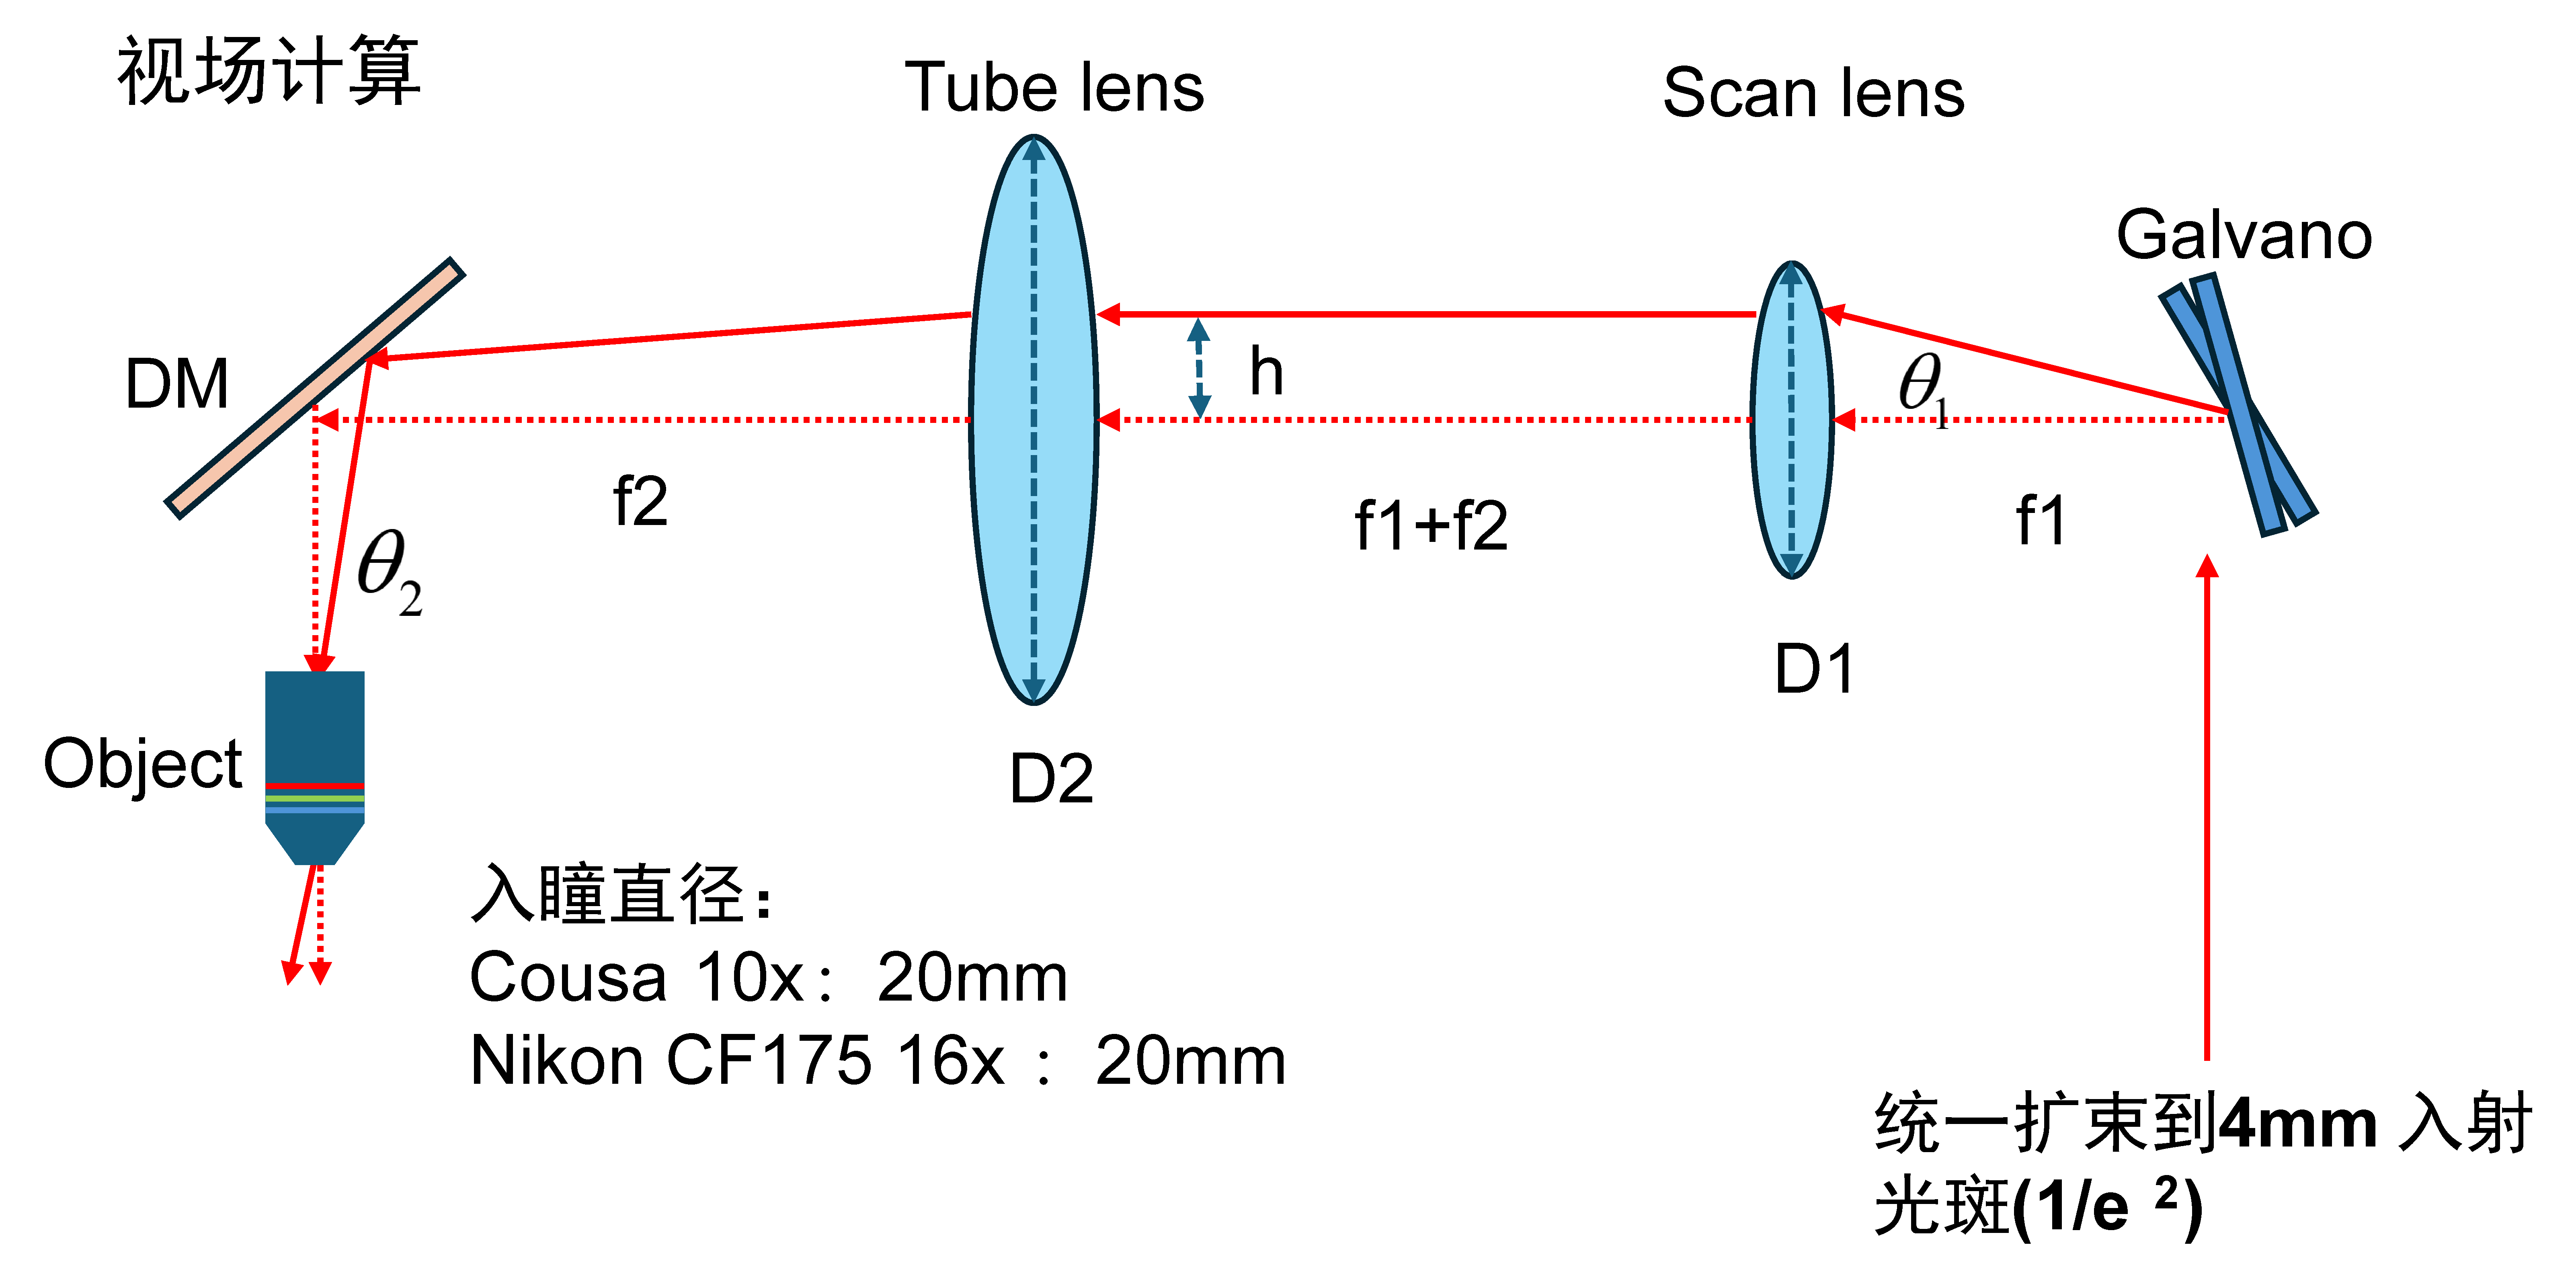
\includegraphics[width=0.85\textwidth]{Fig/Fig3P01}
%     \caption{扫描系统中的扩束设计及视场映射关系示意图}
%     \label{fig3P01}
% \end{figure}

\subsection{扫描视场与分辨率的工程权衡}\label{2.4.4}

对于扫描显微系统而言，视场与分辨率通常并非可以同时无限提升的独立指标，而是受到物镜后孔径、扫描角范围以及中继光学口径共同制约。由式~(\ref{eq:fov_object}) 和式~(\ref{eq:NAeff}) 可见，在扫描角 $\alpha$、扫描透镜焦距 $f_s$ 以及 BFP 处束径 $D_{\mathrm{laser}}$ 给定的情况下，扩大物方视场通常意味着需要更大的扫描角、更大的扫描像圈以及更高通光余量；而提升 $\mathrm{NA}_{\mathrm{eff}}$ 则要求在物镜后孔径处提供更大的束径，并对扩束系统、中继透镜孔径和系统像差控制提出更高要求。

对于本文采用 Olympus XLPLN25XWMP2物镜和Pacific Optica Cousa物镜，一方面其较大的标称 NA 有利于获得较高的激发效率与荧光收集效率；另一方面，其后孔径直径也相应较大，对扩束倍率和扫描系统有效通光孔径提出了更高要求。若扩束不足，则 $\mathrm{NA}_{\mathrm{eff}}$ 下降，系统分辨率无法达到物镜标称水平；若一味追求大视场，则又容易受到视场数、扫描透镜孔径及边缘像差的共同限制。因此，工程实现中通常需要进行均衡设计。

\begin{table}[htbp]
\bicaption{本文实验系统所用 Olympus 25$\times$/1.05 NA 水浸物镜的关键参数}{Key parameters of the Olympus 25$\times$/1.05~NA water-immersion objective used in this work}
\label{tab:olympus_obj}
\centering
\begin{tabular}{|c|c|}
\hline
参数 & 数值 \\ \hline
品牌 & Olympus \\ \hline
标称放大倍率 $M$ & 25$\times$ \\ \hline
标称数值孔径 NA & 1.05 \\ \hline
标准管透镜焦距 $f_{t0}$ & 180 mm \\ \hline
工作距离 $f_0$ & 2 mm \\ \hline
视场数 $D_{\mathrm{BFP}}$ & 18 \\ \hline
系统类型 & 无穷远校正 \\ \hline
\end{tabular}
\end{table}

综上，物镜参数、后孔径束径填充和扫描角度映射共同决定了扫描显微系统的最终性能。对于本文所构建的系统，Olympus 20$\times$/1.05 NA 物镜提供了较高的聚焦和收集能力，而系统可实现的有效视场则进一步受到 180\,mm 管透镜标准、物镜视场数以及扫描光学通光口径的共同约束。因此，在系统设计中需要将``低NA 激发、高NA收集''和``大视场扫描''作为统一的工程优化问题加以权衡。


\subsection{自研物镜设计实例}\label{2.4.5}

为评估在较大扫描视场条件下开展自研物镜设计的可行性，本文进一步在 Zemax 中设计了一支约 12$\times$/0.4 NA 的空气物镜，并采用 CDGM 玻璃库进行了材料替换与优化。需要说明的是，该设计主要用于验证在给定数值孔径、视场范围及国产玻璃约束下的像质可达性，并非本文多光子实验系统中的实际工作物镜，因此本文不进一步展开制造公差与装调误差分析。按照 200 mm 管镜焦距折算，该物镜的等效放大倍率约为 11.84$\times$，有效焦距为 16.894 mm，设计波长为 0.486 $\mu$m、0.588 $\mu$m 和 0.656 $\mu$m，最大视场为 0.8$^\circ$。此外，该系统采用无穷远校正结构，光阑位于第 12 面，总光学长度约为 69.9 mm。

\begin{figure}[htbp]
    \centering
    \begin{subfigure}[b]{0.7\linewidth}
        \centering
        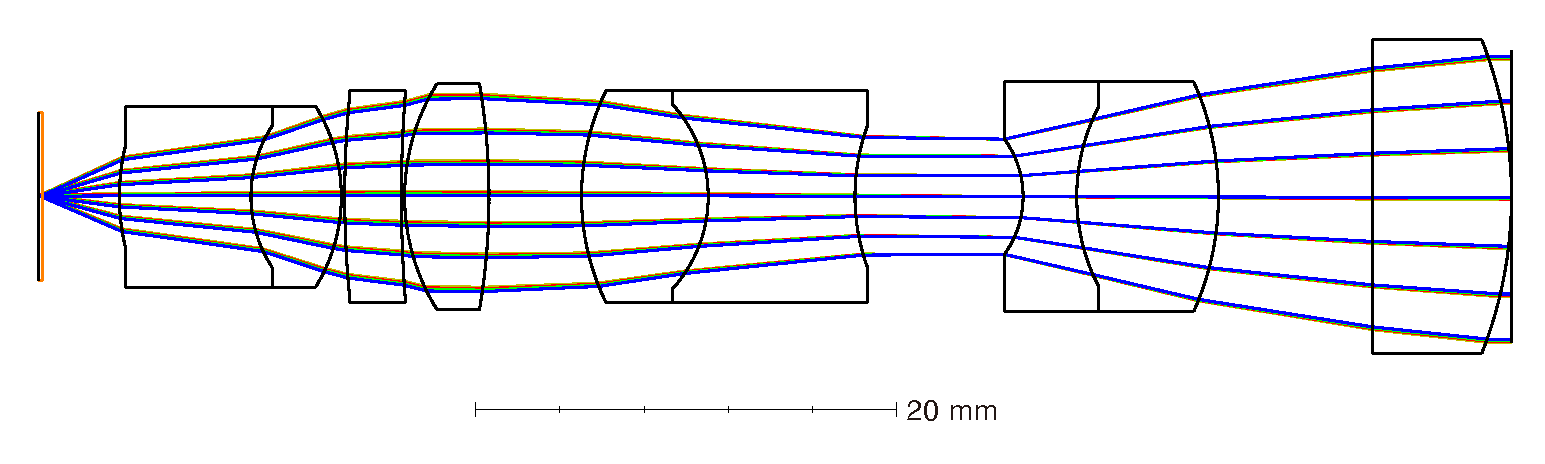
\includegraphics[width=\linewidth]{Fig/Fig-Obj-布局图.pdf}
        \caption{}
        \label{fig_obj_a}
    \end{subfigure}

    \vspace{0.2cm}

    \begin{subfigure}[b]{0.7\linewidth}
        \centering
        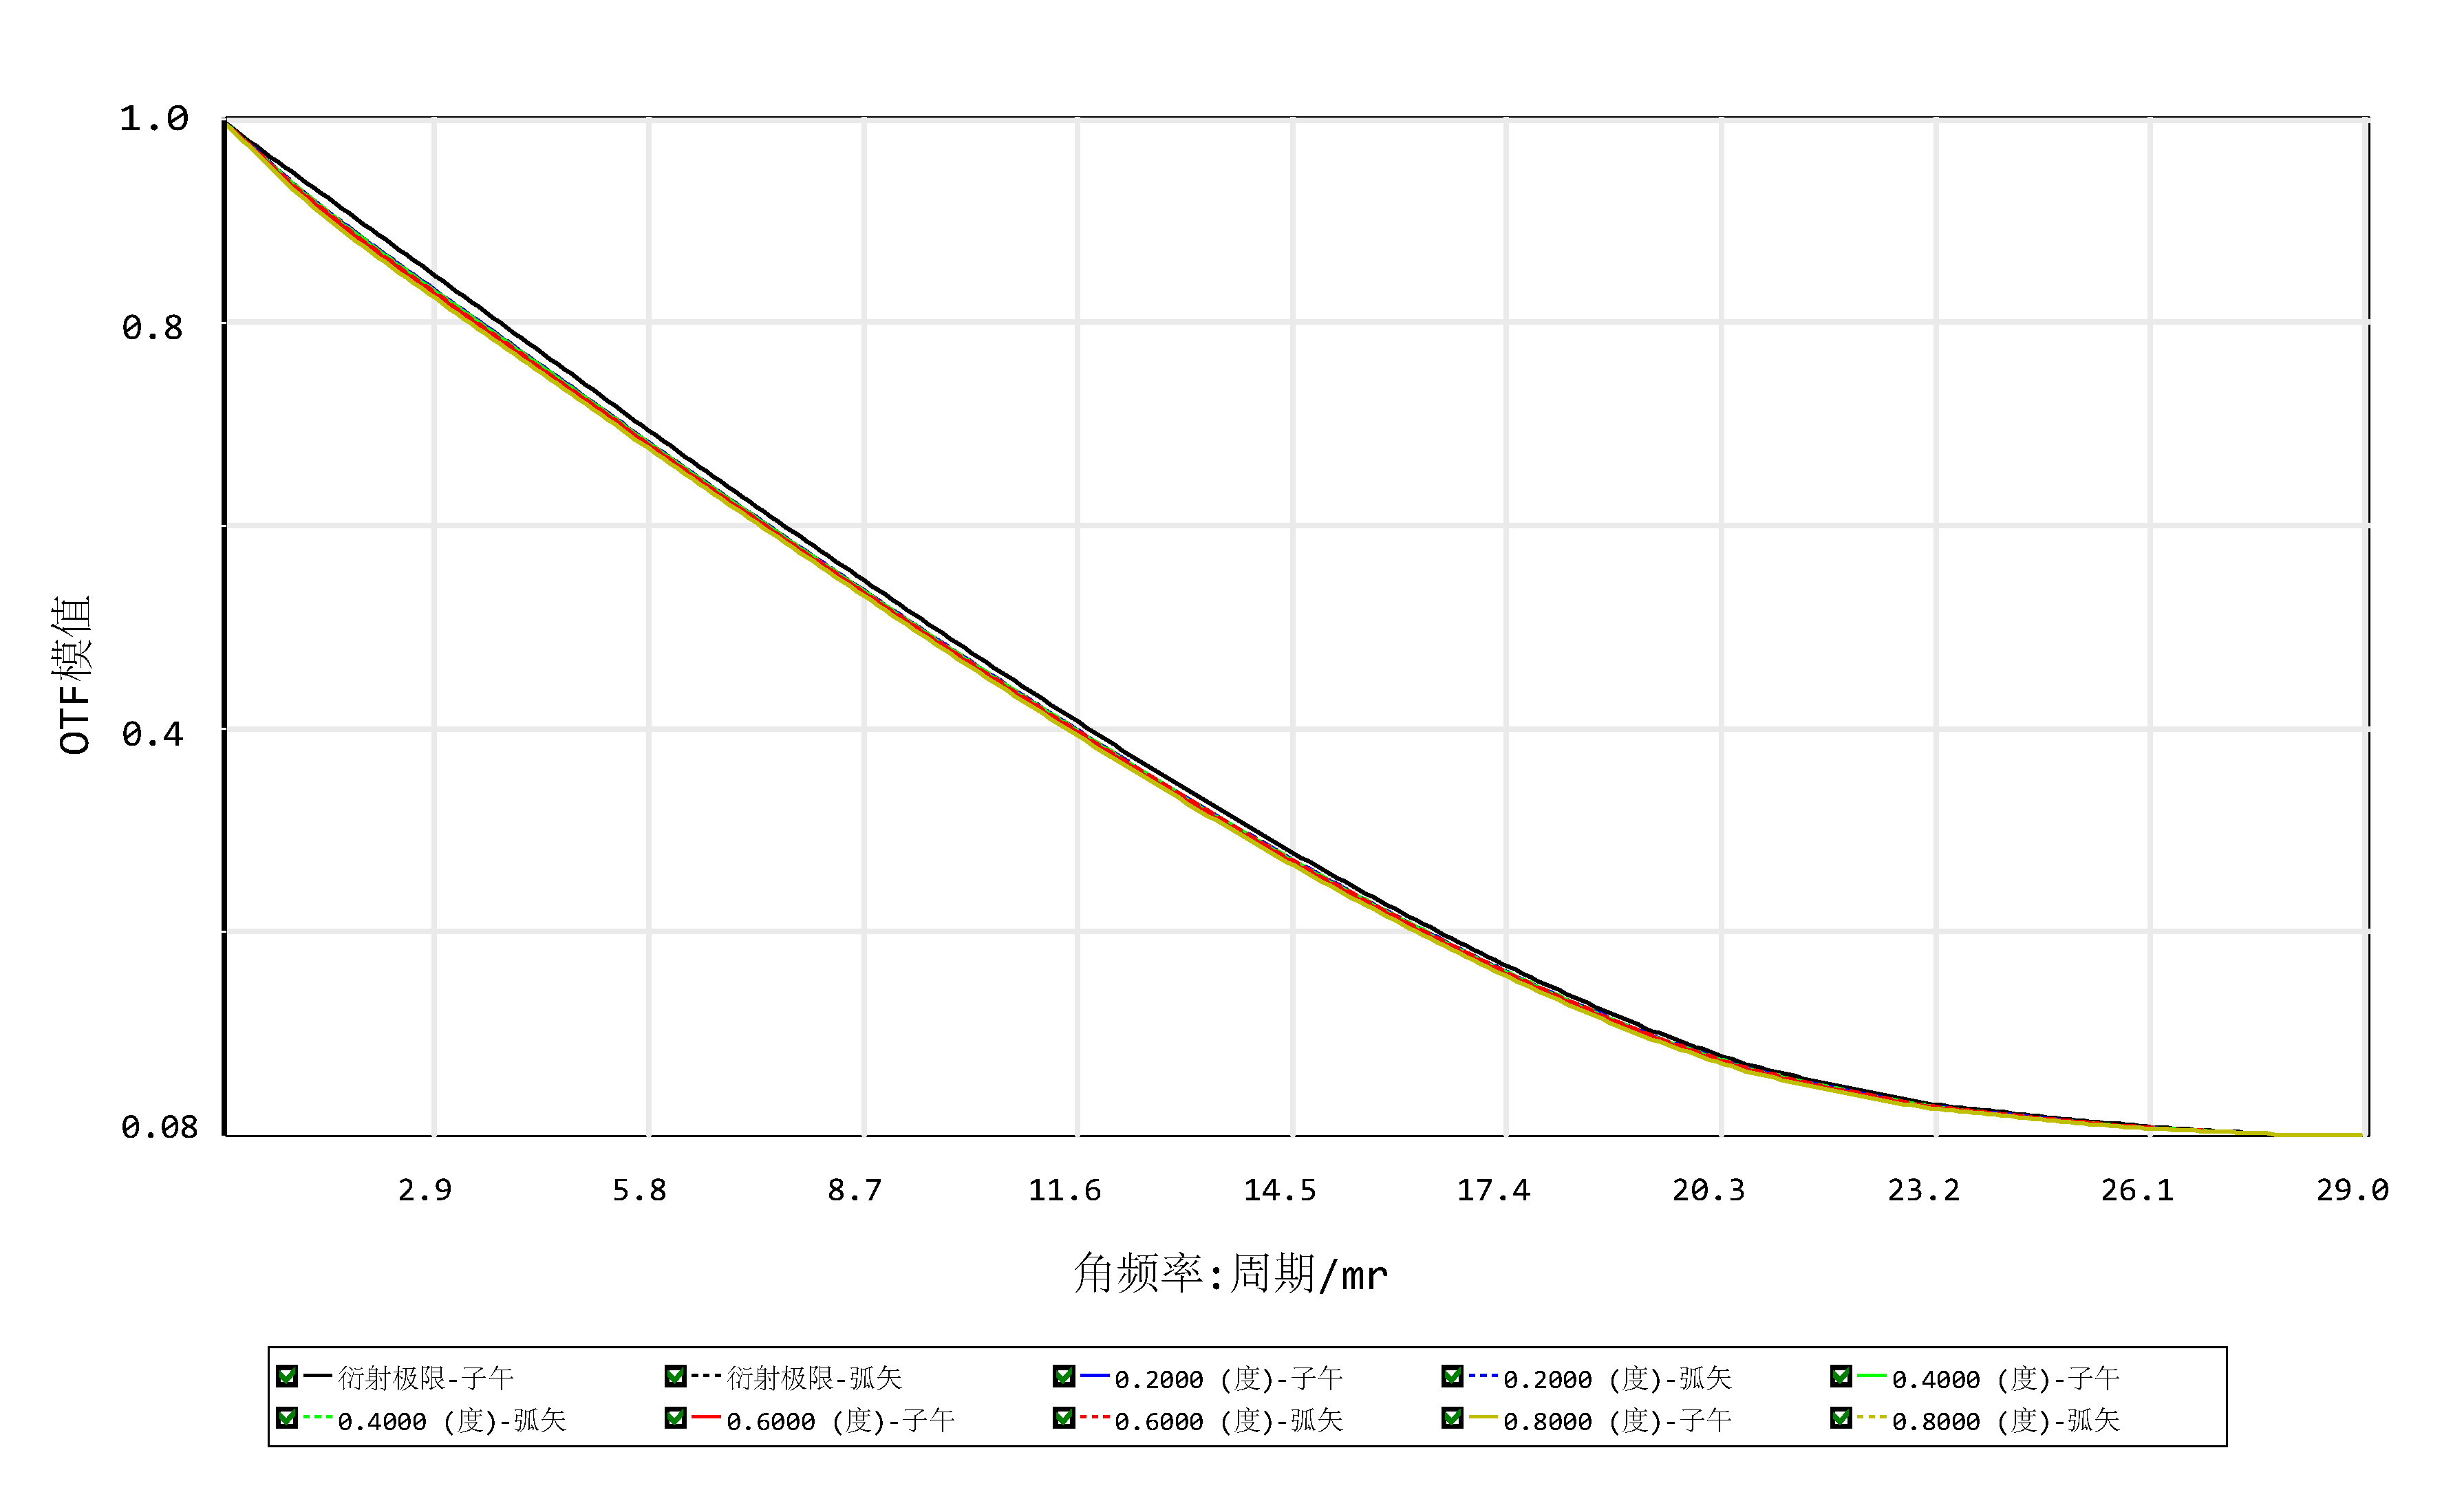
\includegraphics[width=\linewidth]{Fig/Fig-Obj-MTF.pdf}
        \caption{}
        \label{fig_obj_b}
    \end{subfigure}

    \bicaption{自研空气物镜的 Zemax 设计结果。(a)光学布局图；(b)不同视场点下的 MTF 曲线}
    {Zemax design results of the self-designed air objective. (a) Optical layout; (b) MTF curves at different field positions}
    \label{fig_obj_layout_mtf}
\end{figure}


\begin{table}[htbp]
    \centering
    \bicaption{自研空气物镜的主要设计指标}{Main design specifications of the self-designed air objective}
    \label{tab:obj_spec}
    \begin{tabular}{lll}
        \toprule
        参数 & 数值 & 说明 \\
        \midrule
        设计类型 & 无穷远校正空气物镜 & 像方无焦空间 \\
        管镜焦距 & 180 mm & 系统设定值 \\
        等效放大倍率 & $\sim 10\times$ &  $M=f_{\mathrm{tube}}/\mathrm{EFL}$  \\
        物方数值孔径 & 0.4 & 物方空间 NA \\
        有效焦距(EFL) & 16.894 mm & Zemax 仿真数据 \\
        设计波长 & 0.486 / 0.588 / 0.656 $\mu$m & 三波长等权优化 \\
        最大视场 & 0.8$^\circ$ & - \\
        视场点 & 0.2$^\circ$, 0.4$^\circ$, 0.6$^\circ$, 0.8$^\circ$ & - \\
        总光学长度 & 69.907 mm & Zemax 设计数据 \\
        入瞳直径 & 2.796 mm & Zemax 设计数据 \\
        像方 F/\# & 6.042 & Zemax 设计数据 \\
        光阑位置 & 第 12 面 & Zemax 设计数据 \\
        玻璃库 & CDGM\_2025 & 国产玻璃替代 \\
        \bottomrule
    \end{tabular}
\end{table}

图~\ref{fig_obj_layout_mtf}(\subref{fig_obj_a}) 给出了该物镜的光学布局，图~\ref{fig_obj_layout_mtf}(\subref{fig_obj_b}) 给出了不同视场点下的 MTF 曲线。可以看出，在 0.2$^\circ$、0.4$^\circ$、0.6$^\circ$ 和 0.8$^\circ$ 四个视场位置处，子午与弧矢方向的 MTF 曲线整体均较接近衍射极限，说明该设计在设定视场范围内保持了较好的频域传递性能。

图~\ref{fig_obj_spot_fc_dist}(\subref{fig_obj_c}) 给出了不同视场位置的像面点列图结果。随着视场从 0.2$^\circ$ 增加到 0.8$^\circ$，RMS 光斑半径由 178.95 $\mu$m 增加到 218.55 $\mu$m，表明离轴像差虽有上升，但整体变化较为平缓。图~\ref{fig_obj_spot_fc_dist}(\subref{fig_obj_d}) 和图~\ref{fig_obj_spot_fc_dist}(\subref{fig_obj_e}) 分别给出了场曲与畸变分析结果。其中，弧矢场曲约为 0.0010 mm，子午场曲约为 0.0022 mm，最大畸变仅为 0.0014\%，说明在当前视场范围内，该设计在像面弯曲和几何失真方面均得到了较好的控制。

此外，附图~\ref{fig_obj_psf_lsa} 进一步给出了 FFT PSF 截面及轴向像差分析结果，为该物镜在波动光学层面的成像质量提供了补充说明。

需要指出的是，本文给出的自研空气物镜主要作为面向特定系统约束的设计实例，用于验证在给定视场范围、结构长度和像质要求下开展定制化物镜设计的可行性。该设计在设定视场内表现出较好的频域传递性能，并实现了较低的场曲和畸变，说明其在目标参数范围内具备接近衍射极限的成像能力。然而，本文尚未将其与 Olympus、Nikon 等成熟商用高数值孔径水浸物镜进行同平台定量比较，因此并不主张该设计在数值孔径、深层组织成像能力或工业成熟度方面优于商用高端物镜。相较于标准化商用品，该类自研设计的主要优势在于可针对特定激发波段、实验室现有管透镜参数以及具体扫描系统结构进行协同优化，从而为后续面向专用场景的定制化显微系统开发提供设计基础。

\begin{figure}[htbp]
    \centering

    \begin{subfigure}[b]{0.9\linewidth}
        \centering
        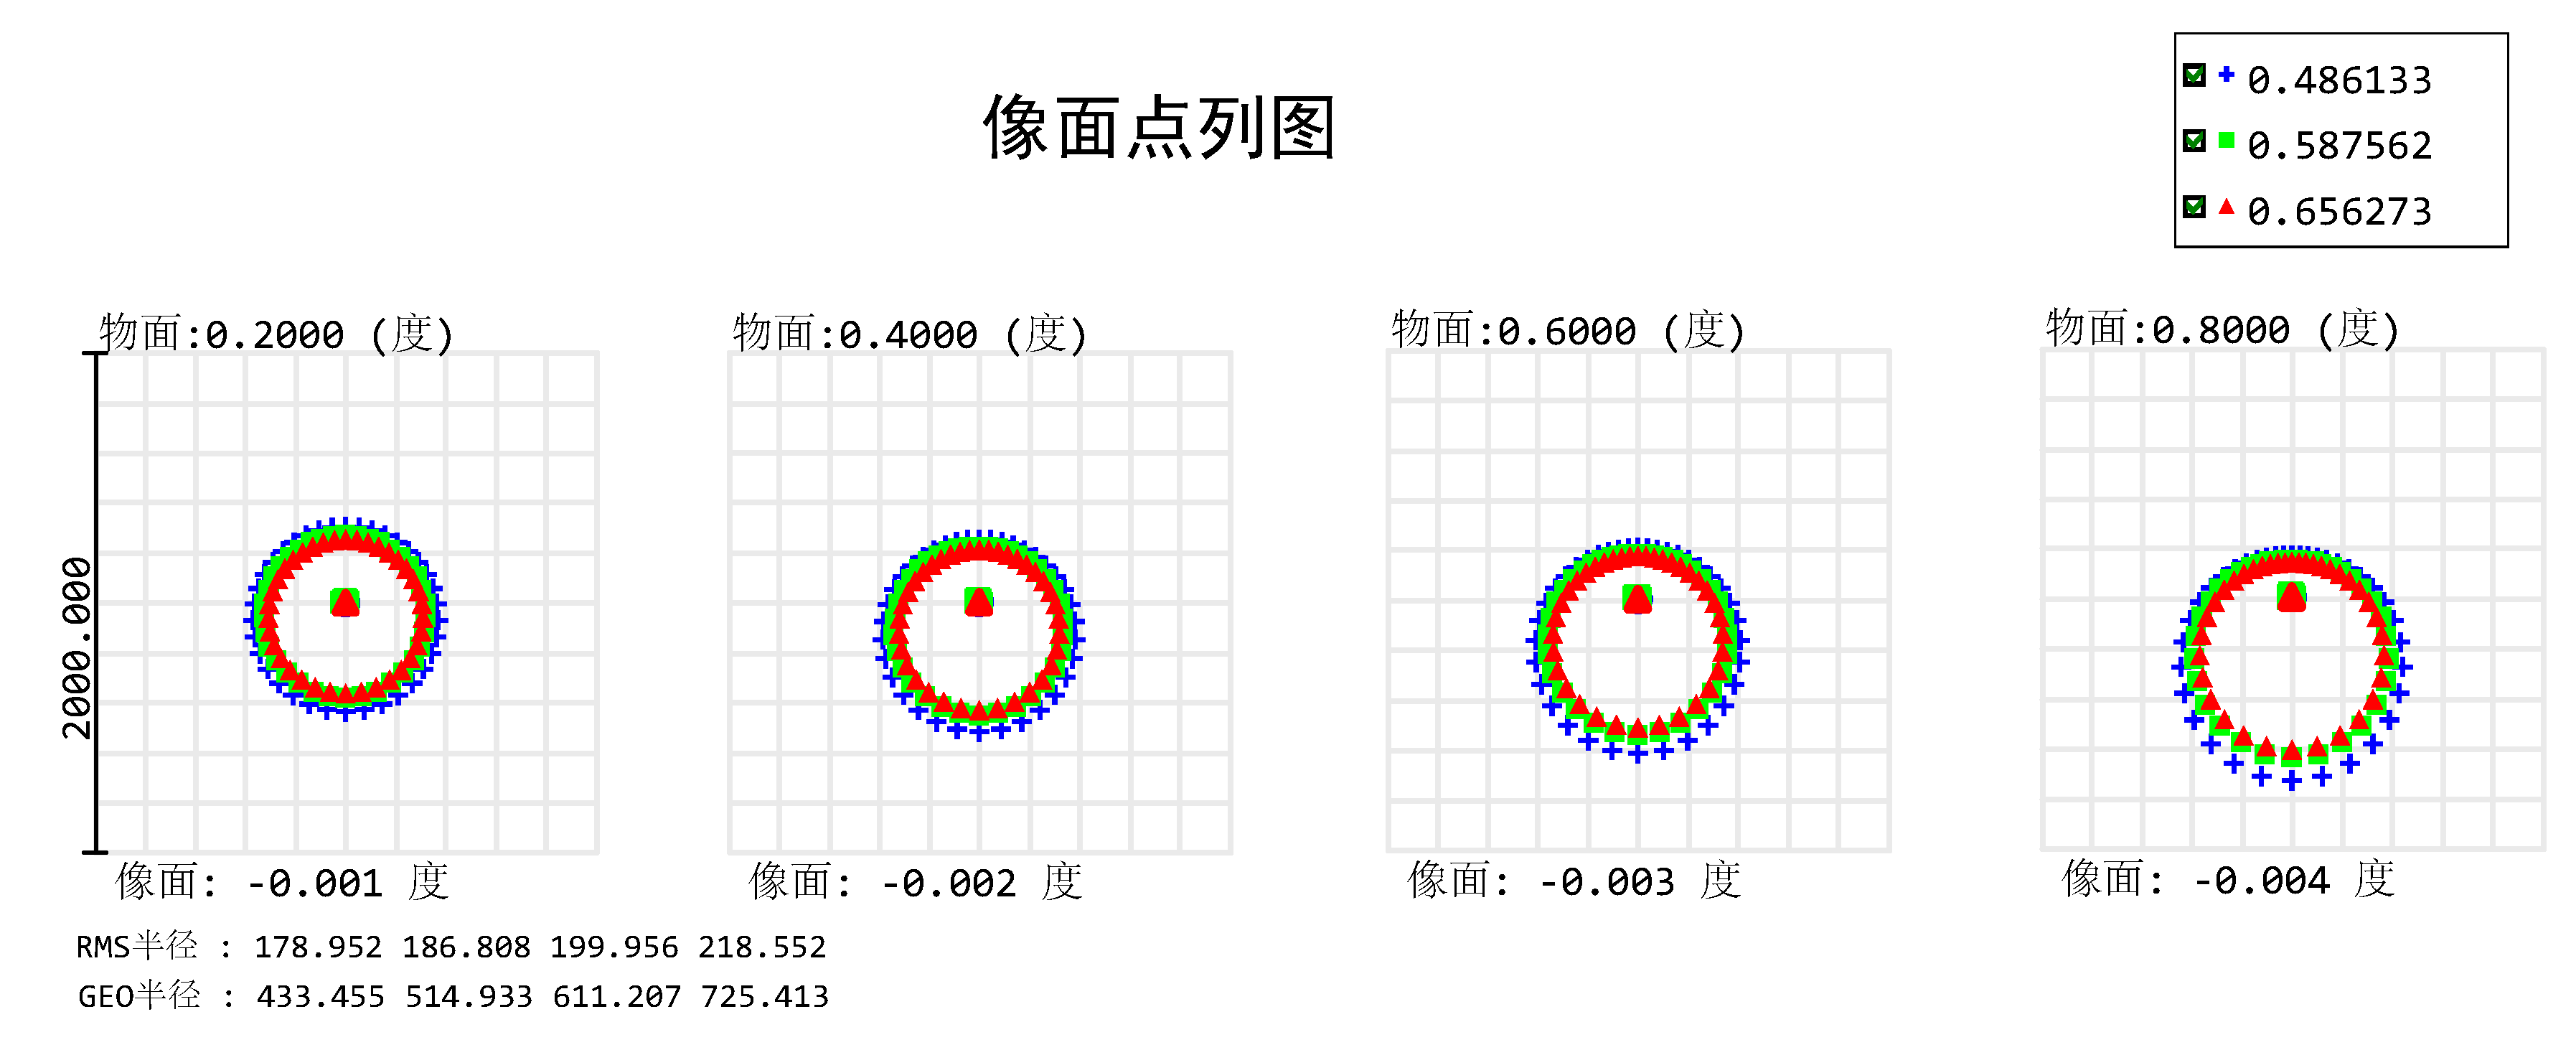
\includegraphics[width=\linewidth]{Fig/Fig-Obj-点列图.pdf}
        \caption{}
        \label{fig_obj_c}
    \end{subfigure}
    \vspace{0.25cm}
    \begin{subfigure}[b]{0.4\linewidth}
        \centering
        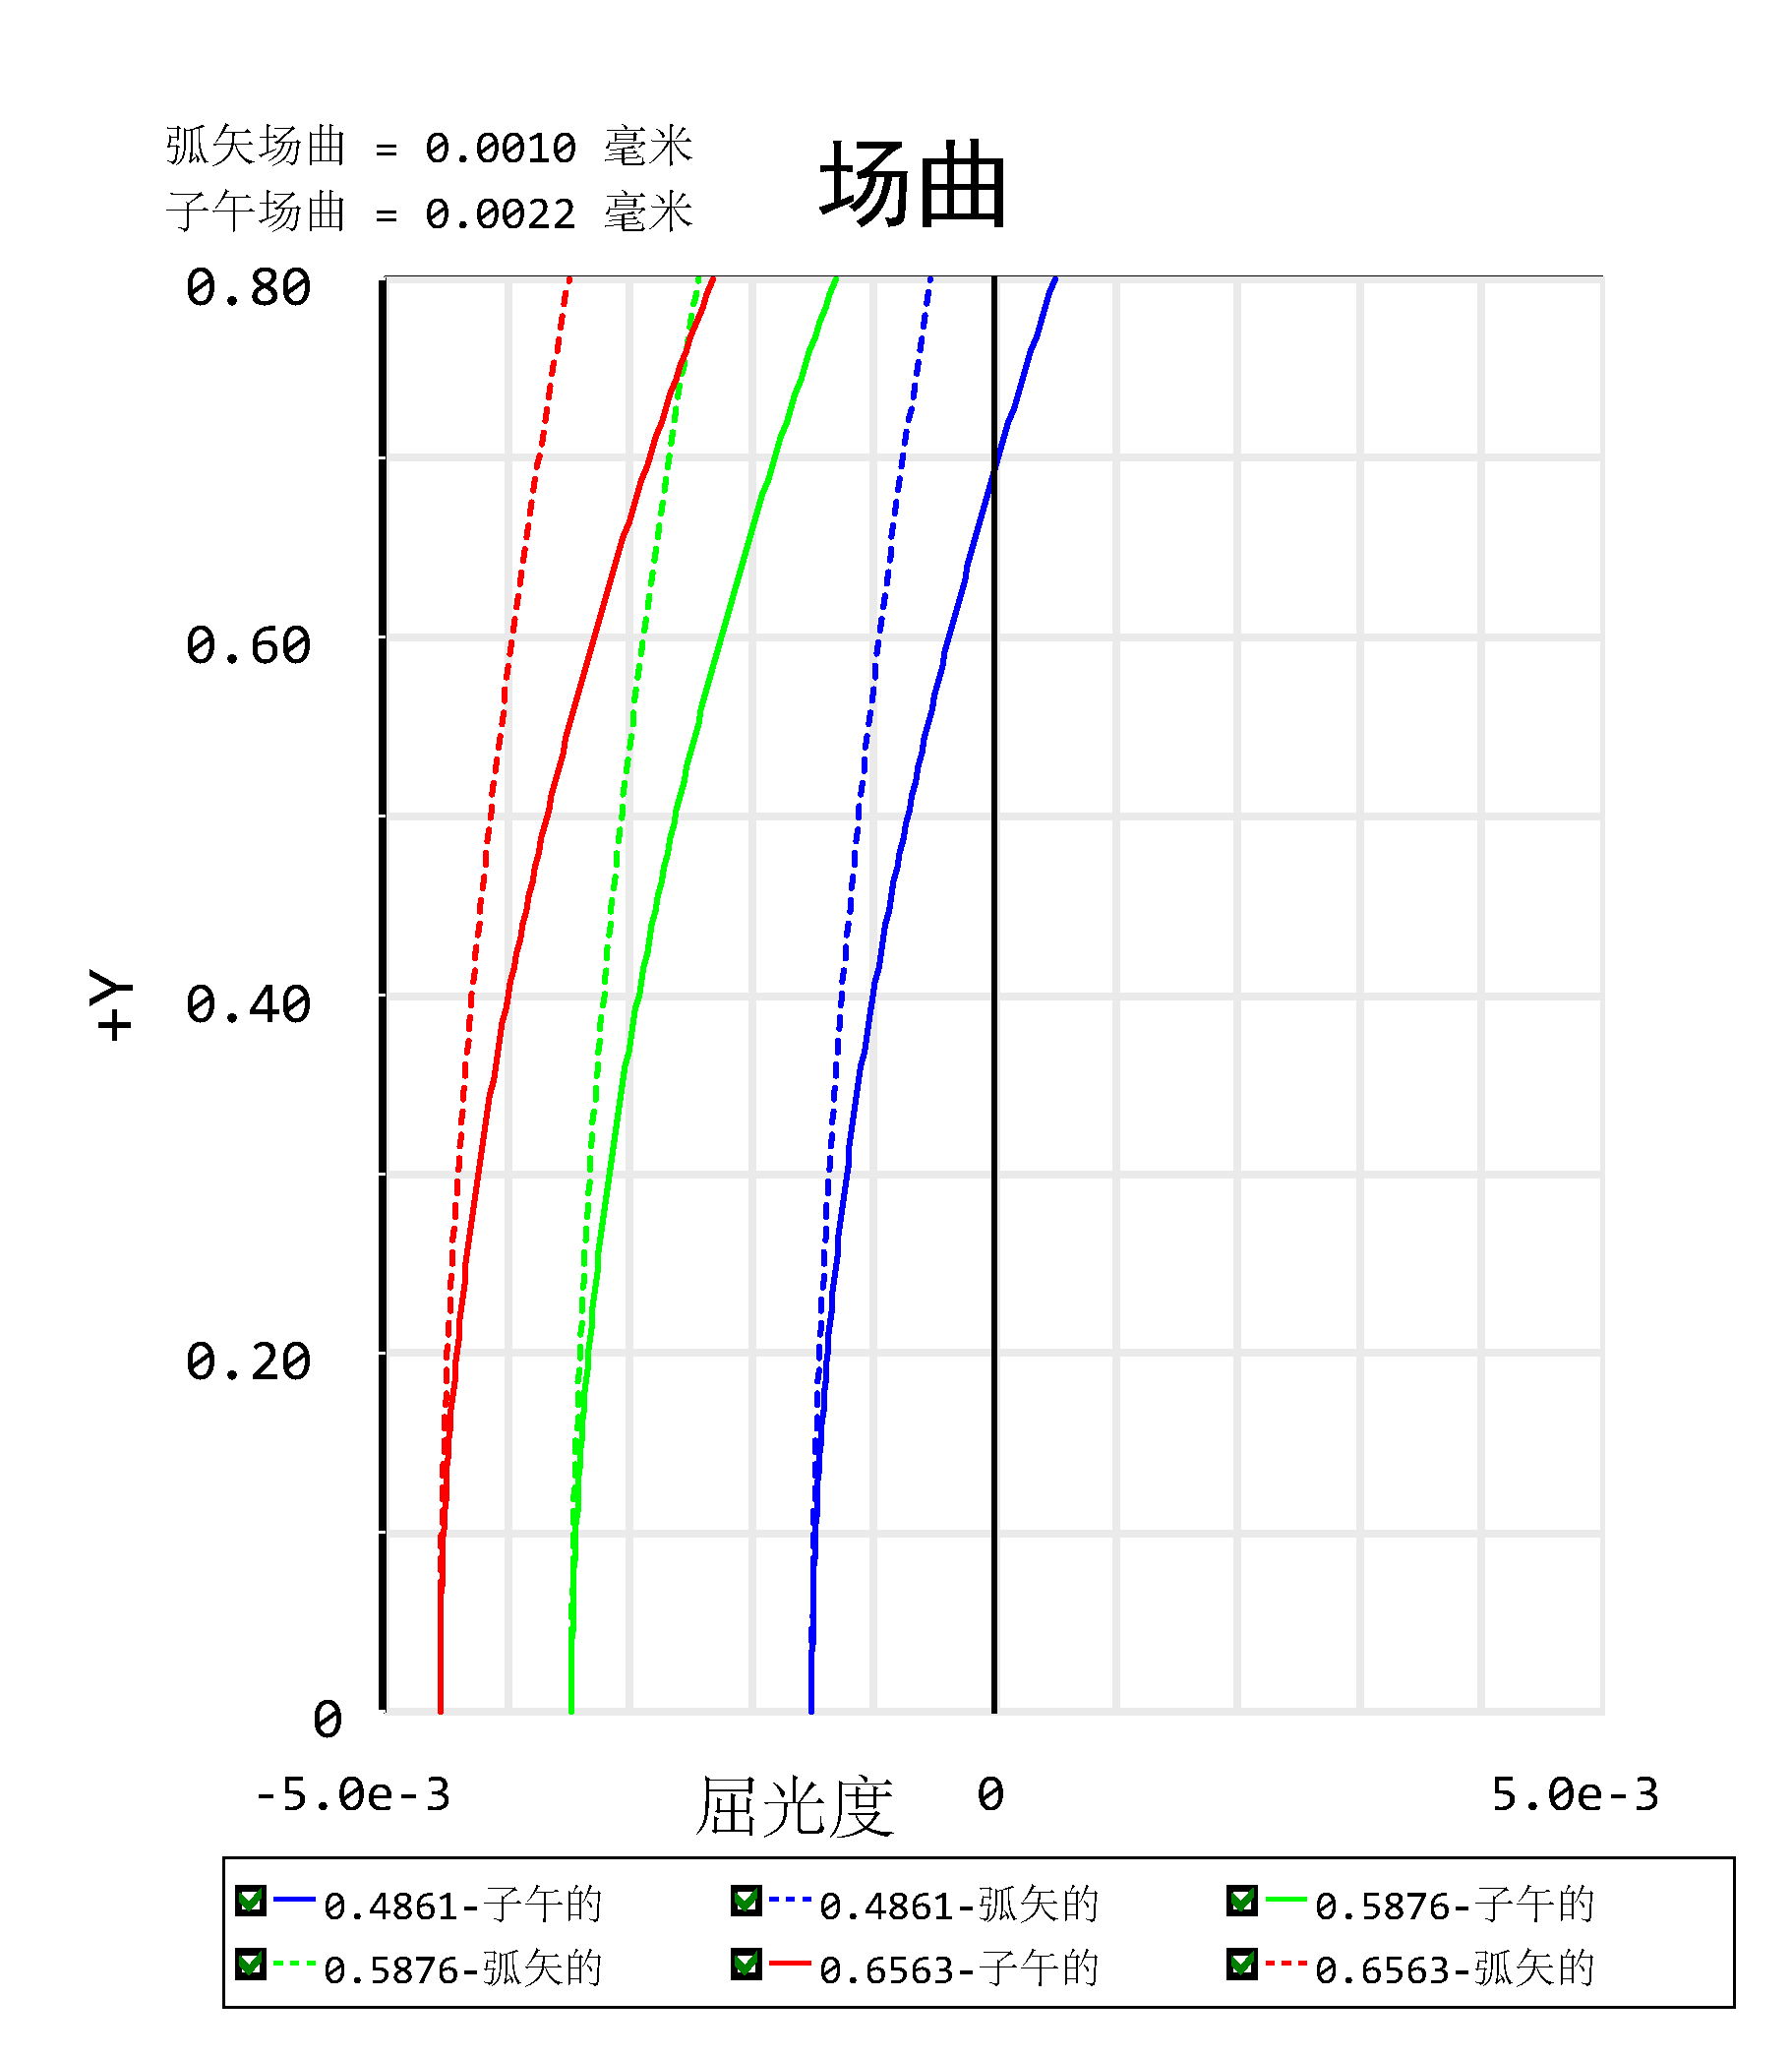
\includegraphics[width=\linewidth]{Fig/Fig-Obj-场曲畸变.pdf}
        \caption{}
        \label{fig_obj_d}
    \end{subfigure}
    \hfil
    \begin{subfigure}[b]{0.4\linewidth}
        \centering
        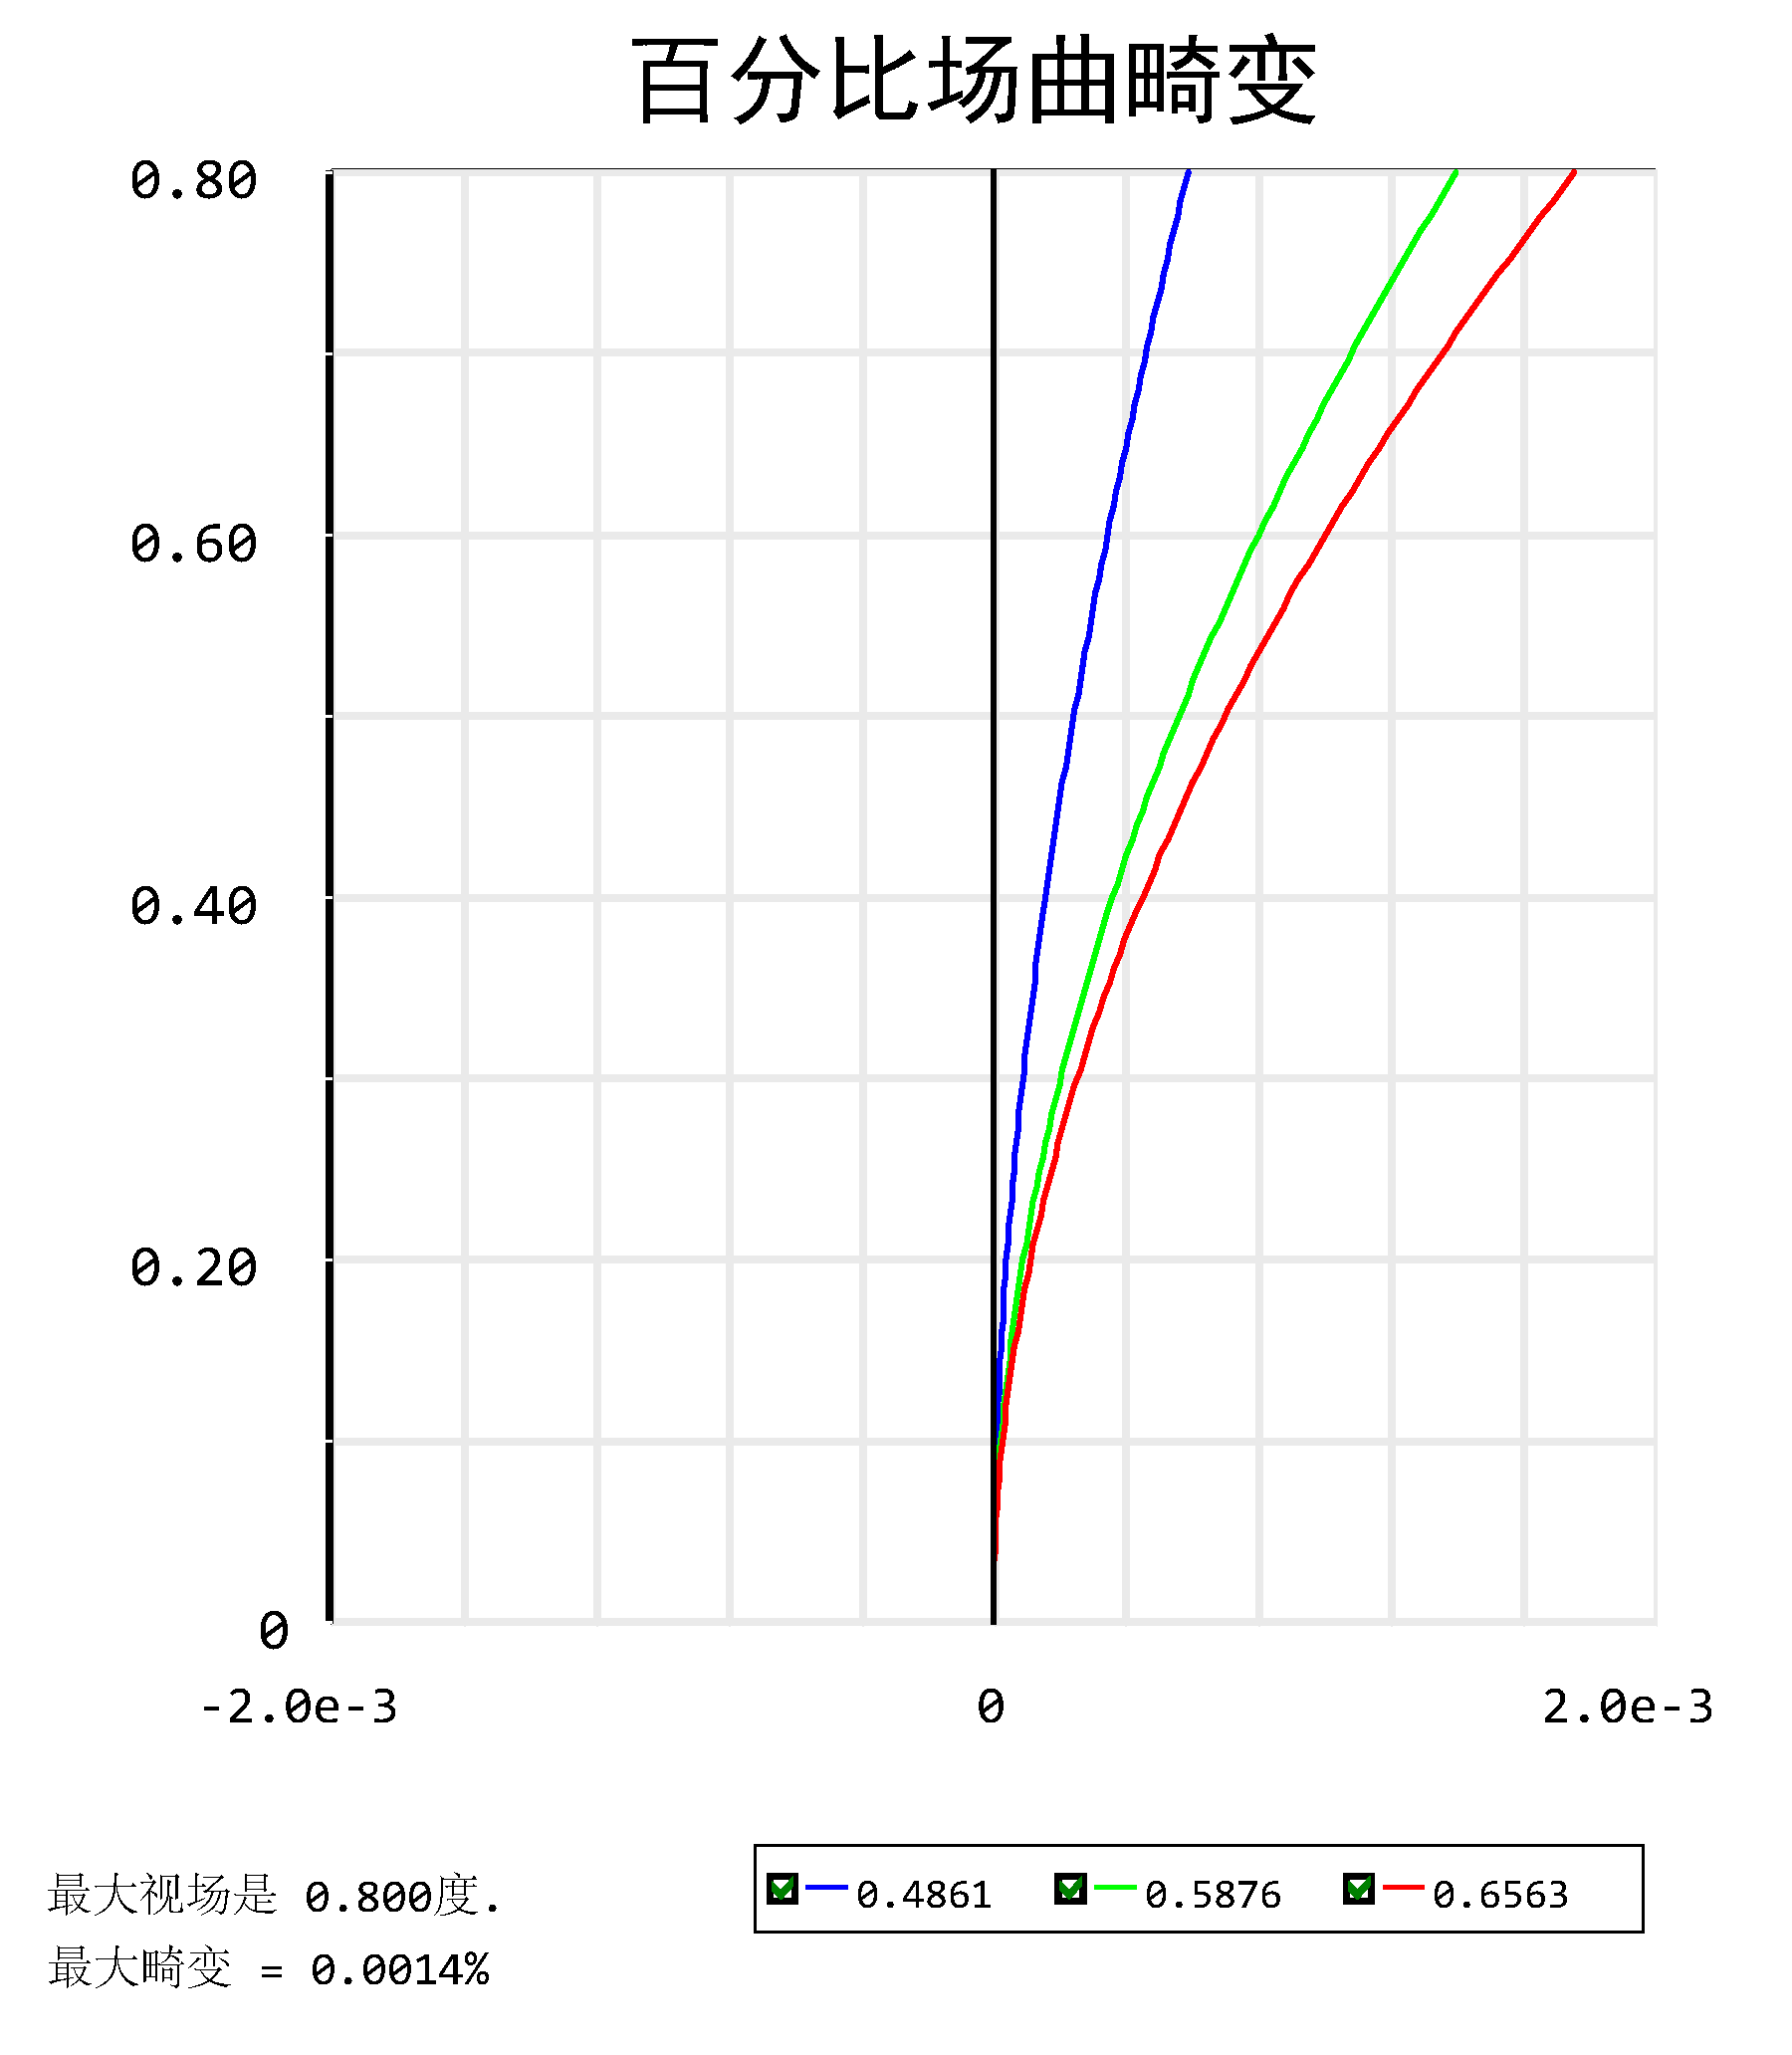
\includegraphics[width=\linewidth]{Fig/Fig-Obj-场曲畸变-百分比.pdf}
        \caption{}
        \label{fig_obj_e}
    \end{subfigure}

    \bicaption{自研空气物镜的离轴像质分析结果。(a)不同视场位置的像面点列图；(b)场曲分析结果；(c)畸变百分比分析结果}
    {Off-axis image-quality analysis of the self-designed air objective. (a) Spot diagrams at different field positions; (b) field curvature; (c) percentage distortion}
    \label{fig_obj_spot_fc_dist}
\end{figure}


\begin{table}[htbp]
    \centering
    \bicaption{自研空气物镜的简化处方参数}{Simplified prescription of the self-designed air objective}
    \label{tab:obj_prescription}
    \begin{tabular}{cccccc}
        \toprule
        面号 & 曲率半径 / mm & 厚度 / mm & 材料 & 净口径 / mm & 备注 \\
        \midrule
        2  & 10.2485  & 6.2622 & H-ZLAF2A & 4.7975  & 折射面 \\
        3  & 6.1201   & 4.2994 & H-FK95N  & 6.7196  & 折射面 \\
        5  & 48.9115  & 2.6964 & H-ZK10L  & 9.3400  & 折射面 \\
        7  & 10.1474  & 4.0144 & D-FK95-25 & 10.7598 & 折射面 \\
        9  & 11.5002  & 6.0277 & H-FK95N  & 10.0682 & 折射面 \\
        10 & -6.5179  & 6.9845 & D-K9GT   & 8.7767  & 折射面 \\
        12 & -4.6773  & 2.5528 & H-K5     & 5.5076  & 光阑所在面 \\
        13 & 9.3071   & 6.7420 & D-FK61   & 8.4923  & 折射面 \\
        15 & 686.2102 & 6.6326 & H-FK95N  & 13.7028 & 近似平面折射面 \\
        16 & -20.3797 & 0       & ---      & 14.9117 & 像前最后一面 \\
        \bottomrule
    \end{tabular}
\end{table}


\begin{table}[htbp]
    \centering
    \bicaption{自研空气物镜在不同视场下的像质指标}{Image-quality metrics of the self-designed air objective at different field positions}
    \label{tab:obj_performance}
    \begin{tabular}{ccccc}
        \toprule
        视场角 / $^\circ$ & RMS光斑半径 / $\mu$m & 最大光斑半径 / $\mu$m & 像坐标 / deg & 备注 \\
        \midrule
        0.2 & 178.95 & 433.46 & -0.00105 & 近轴视场 \\
        0.4 & 186.81 & 514.93 & -0.00210 & 中间视场 \\
        0.6 & 199.96 & 611.21 & -0.00316 & 中间视场 \\
        0.8 & 218.55 & 725.41 & -0.00421 & 边缘视场 \\
        \midrule
        \multicolumn{5}{l}{弧矢场曲：0.0010 mm；子午场曲：0.0022 mm；最大畸变：0.0014\%} \\
        \bottomrule
    \end{tabular}
\end{table}



